
\documentclass[12pt,a4paper]{report}
\usepackage[utf8]{inputenc}
\usepackage[T1]{fontenc}
\usepackage{geometry,graphicx,amsmath,amssymb,booktabs,array,tabularx,float}
\usepackage{fancyhdr,xcolor,setspace,enumitem,caption,subcaption,multirow,colortbl}
\usepackage{longtable,titlesec,titletoc,lastpage,makecell,etoolbox,needspace}
\usepackage[hidelinks]{hyperref}
\numberwithin{table}{chapter}
\numberwithin{figure}{chapter}
\newcommand{\placeholder}[1]{\textit{\textless #1\textgreater}}
\newcommand{\todo}[1]{\colorbox{yellow}{TODO: #1}}
\newcolumntype{L}[1]{>{\raggedright\arraybackslash}p{#1}}
\newcolumntype{C}[1]{>{\centering\arraybackslash}p{#1}}
\newcolumntype{R}[1]{>{\raggedleft\arraybackslash}p{#1}}
\newcommand{\sdstar}{\textsuperscript{*}}
\newcommand{\reportProject}{DEMONSTRATION ONLY - synthetic bridge results}
\newcommand{\reportJob}{DEMO-001}
\newcommand{\reportDate}{2026-11-17}
\newcommand{\reportVersion}{Synthetic data - no structural analysis}

% All presentation settings originate in reports/styles.py.
\geometry{a4paper,left=2.0cm,right=2.0cm,top=2.0cm,bottom=2.0cm,
  includeheadfoot,headheight=30.0pt,headsep=10pt,footskip=32.0pt}
\definecolor{osdagGreen}{HTML}{91B014}
\definecolor{reportFail}{HTML}{B33724}
\definecolor{reportWarning}{HTML}{1D5B8F}
\definecolor{reportText}{HTML}{263238}
\color{reportText}
\setstretch{1.12}
\setlength{\parindent}{0pt}
\setlength{\emergencystretch}{2em}
\captionsetup{labelfont=bf,justification=raggedright,singlelinecheck=false,
  format=plain,font=small,skip=5pt}
\newcommand{\ReportCaptionSetup}{%
  \setlength{\abovecaptionskip}{5pt}\setlength{\belowcaptionskip}{5pt}}
\newcommand{\ReportTableSetup}{%
  \setlength{\tabcolsep}{3.0pt}%
  \renewcommand{\arraystretch}{1.18}%
  \setlength{\arrayrulewidth}{0.4pt}\setlength{\extrarowheight}{0.5pt}%
  \setlength{\LTleft}{\fill}\setlength{\LTright}{\fill}%
  \setlength{\LTpre}{4pt}\setlength{\LTpost}{8pt}}
\newcommand{\ReportTableFont}{\small}
\newcommand{\ReportSmallText}{\footnotesize}
\newcommand{\ReportExecutiveTitle}{\centering\Large\bfseries}
\newcommand{\ReportRowGap}{3.0pt}
\newcommand{\ReportTableGap}{\vspace{0.5em}}
\newcommand{\ReportSectionGap}{\vspace{0.8em}}
\newcommand{\ReportCellGap}{\vspace{3pt}}
\newcommand{\ReportChapterFormat}{%
  \titleformat{\chapter}[block]{\normalfont\Large\bfseries\centering}%
    {\thechapter}{1em}{}%
  \titlespacing*{\chapter}{0pt}{0pt}{10pt}}
\ReportChapterFormat
\BeforeBeginEnvironment{longtable}{\Needspace{6\baselineskip}}
\newcommand{\ReportPageFurniture}{%
  \fancyhf{}%
  \fancyhead[L]{\parbox[b]{0.48\headwidth}{\scriptsize\raggedright\reportProject\ $|$ \reportJob}}%
  \fancyhead[R]{\parbox[b]{0.48\headwidth}{\scriptsize\raggedleft\reportDate\ $|$ \reportVersion}}%
  \fancyfoot[L]{\scriptsize Osdag $|$ FOSSEE $|$ Indian Institute of Technology Bombay}%
  \fancyfoot[R]{\scriptsize Page \thepage\ of \pageref{LastPage}}%
  \renewcommand{\headrulewidth}{0.6pt}%
  \renewcommand{\footrulewidth}{0.6pt}%
  \renewcommand{\headrule}{\hbox to\headwidth{\color{osdagGreen}\leaders\hrule height 0.6pt\hfill}}%
  \renewcommand{\footrule}{\hbox to\headwidth{\color{osdagGreen}\leaders\hrule height 0.6pt\hfill}}}
\fancypagestyle{main}{\ReportPageFurniture}
\fancypagestyle{plain}{\ReportPageFurniture}
\fancypagestyle{firstpage}{\ReportPageFurniture\fancyhead{}\renewcommand{\headrulewidth}{0pt}}
\pagestyle{main}
\setcounter{tocdepth}{2}
\titlecontents{chapter}[1.5em]{\normalfont\vspace{2pt}}{\contentslabel{1.5em}}{\hspace*{-1.5em}}{\hfill\contentspage}
\titlecontents{section}[3.8em]{\normalfont}{\contentslabel{2.3em}}{\hspace*{-2.3em}}{\hfill\contentspage}
\titlecontents{subsection}[7em]{\normalfont}{\contentslabel{3.2em}}{\hspace*{-3.2em}}{\hfill\contentspage}
\renewcommand{\contentsname}{\centering\Large\bfseries Table of Contents}

\begin{document}


\begin{titlepage}
\thispagestyle{firstpage}
\centering
\vspace*{1.5cm}
\noindent
\begin{minipage}[c]{0.6\textwidth}
\raggedright

\includegraphics[width=\linewidth,keepaspectratio]{Report_After_assets/osdag_logo.png}
\end{minipage}%
\hfill
\begin{minipage}[c]{0.35\textwidth}
\raggedleft

\end{minipage}
\\[1cm]

{\Huge \textbf{OsdagBridge}}\\[0.3cm]
{\large Open Source Software for Steel Girder Bridge Design}\\[1.5cm]
{\Large Design Report}\\[1.5cm]
\begingroup
\ReportTableSetup
\ReportTableFont
\begin{longtable}{|L{4.0000cm}|L{10.0000cm}|}
\hline
\textbf{Parameter} & \textbf{Value} \\
\hline
\endfirsthead
\hline
\textbf{Parameter} & \textbf{Value} \\
\hline
\endhead
\hline
\endfoot
\hline
\endlastfoot

\textbf{Project Name} & DEMONSTRATION ONLY - synthetic bridge results \\
\hline
\textbf{Project Location} & Sample location \\
\hline
\textbf{Author / Designer} & Report rendering demonstration \\
\hline
\textbf{Reviewer} & N/A \\
\hline
\textbf{Organization} & OsdagBridge screening exercise \\
\hline
\textbf{Client Name and Organization} & Not for construction \\
\hline
\textbf{Job Number} & DEMO-001 \\
\hline
\textbf{Date} & 2026-11-17 \\
\hline
\textbf{Report Version} & Synthetic data - no structural analysis \\
\hline
\end{longtable}
\endgroup
\end{titlepage}
\setcounter{page}{2}

\clearpage\tableofcontents

\newpage
{\ReportExecutiveTitle Executive Summary\par}
\addcontentsline{toc}{chapter}{Executive Summary}
\ReportTableGap

This section provides a concise summary of the bridge design, key inputs, governing loads, and final design outcomes.

\section*{Project Overview}
\addcontentsline{toc}{section}{Project Overview}
\label{sec:project-overview}


\begingroup
\ReportTableSetup
\ReportTableFont
\begin{longtable}{|L{5.5000cm}|L{8.5000cm}|}
\hline
\textbf{Parameter} & \textbf{Value} \\
\hline
\endfirsthead
\hline
\textbf{Parameter} & \textbf{Value} \\
\hline
\endhead
\hline
\endfoot
\hline
\endlastfoot

\textbf{Bridge Type} & N/A \\
\hline
\textbf{Design Standard} & IRC 5, IRC 6, IRC 22, IRC 24, IS 800 \\
\hline
\textbf{Span} & 25 m \\
\hline
\textbf{Carriageway Width} & N/A \\
\hline
\textbf{No. of Girders} & 4 \\
\hline
\textbf{Girder Spacing} & 2.5 \\
\hline
\textbf{Deck Thickness} & 250 \\
\hline
\textbf{Overall Design Status} & Exceeds UR limit \\
\hline
\textbf{Governing Check} & End diaphragms \\
\hline
\textbf{Overall Utilization Ratio (max)} & 1.15 (End diaphragms) \\
\hline
\end{longtable}
\endgroup


\noindent\textit{Unavailable: Figure 1 -- Overall Bridge Plan. No drawing was supplied.}\par


\ReportTableGap

\noindent\textit{Unavailable: Figure 2 -- Typical Cross-Section (with girder, deck, barriers, footpath). No drawing was supplied.}\par


\noindent\textit{Unavailable: Figure 3 -- 3D View of Bridge Superstructure. No drawing was supplied.}\par


\begingroup
\ReportTableSetup
\ReportTableFont
\begin{longtable}{|L{1.8000cm}|L{2.8000cm}|L{6.0000cm}|C{1.6000cm}|C{2.0000cm}|}
\caption{Reported Girder Summary}\\\hline
\textbf{Member} & \textbf{Member ID} & \textbf{Governing reported check} & \textbf{UR} & \textbf{Backend status} \\ \hline
\endfirsthead
\hline
\textbf{Member} & \textbf{Member ID} & \textbf{Governing reported check} & \textbf{UR} & \textbf{Backend status} \\ \hline
\endhead
\hline
\endfoot
\hline
\endlastfoot

G1 & G1M1 & Flexure (synthetic) & 0.72 & PASS \\ \hline
G2 & G2M1 & Flexure (synthetic) & 0.88 & PASS \\ \hline
G3 & G3M1 & Flexure (synthetic) & 1.08 & FAIL \\ \hline
G4 & G4M1 & Flexure (synthetic) & 0.93 & WARN \\ \hline
\end{longtable}
\endgroup
\textit{Controlling-girder section designation (legacy reference): N/A.}

\ReportTableGap
\noindent\textit{Note: Utilization ratio (UR) = demand / capacity. The chart reference limit is $1.0$. Missing results remain unavailable; review each engine check and status.}

\ReportTableGap

\section*{Key Design Outcomes Summary}
\addcontentsline{toc}{section}{Key Design Outcomes Summary}
\label{sec:key-outcomes}

\noindent Steel plate girders:\allowbreak{} Exceeds UR limit; maximum UR 1.08\\
Concrete deck slab:\allowbreak{} Within UR limit (reported checks); maximum UR 0.77\\
Cross bracing:\allowbreak{} Within UR limit (reported checks); maximum UR 0.50\\
End diaphragms:\allowbreak{} Exceeds UR limit; maximum UR 1.15\\
Backend WARN statuses are present; review the detailed checks.\\
Backend FAIL statuses are present; a numeric chart limit does not override them.

\section*{Design Assumptions and Limitations}
\addcontentsline{toc}{section}{Design Assumptions and Limitations}
\label{sec:assumptions}

\begin{itemize}
\item Additional inputs not provided by the user were assumed by software per IRC/IS code defaults or practical consideration.
\item This document renders supplied results. Generating a report does not run or validate a structural analysis.
\item Substructure and foundation design are not included in this report.
\item Splice connections and bearings are not designed in this version.
\end{itemize}

% Restore numbered chapter format
\ReportChapterFormat


\chapter{Project Information}

This section records all project metadata as entered by the designer.

\section{Project and Design Team Details}
\label{sec:project-details}

\begingroup
\ReportTableSetup
\ReportTableFont
\begin{longtable}{|L{5.5000cm}|L{8.5000cm}|}
\hline
\textbf{Parameter} & \textbf{Value} \\
\hline
\endfirsthead
\hline
\textbf{Parameter} & \textbf{Value} \\
\hline
\endhead
\hline
\endfoot
\hline
\endlastfoot

\textbf{Project Name} & DEMONSTRATION ONLY - synthetic bridge results \\
\hline
\textbf{Project Location} & Sample location \\
\hline
\textbf{Designer} & Report rendering demonstration \\
\hline
\textbf{Reviewer} & N/A \\
\hline
\textbf{Organization} & OsdagBridge screening exercise \\
\hline
\textbf{Client} & Not for construction \\
\hline
\textbf{Software Version} & OsdagBridge \\
\hline
\end{longtable}
\endgroup


\section{Applicable Codes and Standards}
\label{sec:codes}

\begin{itemize}
\item Indian Roads Congress (IRC) 5: General Features of Design
\item Indian Roads Congress (IRC) 6: Loads and Load Combinations
\item Indian Roads Congress (IRC) 22: Composite Construction (Limit State Design)
\item Indian Roads Congress (IRC) 24: Steel Road Bridges (Limit State Method)
\item Indian Roads Congress (IRC) 112: Concrete Road Bridges (deck design)
\item Indian Roads Congress Special Publication (IRC SP) 114: Seismic Design of Road Bridges
\item Indian Standard (IS) 800: General Construction in Steel
\item Indian Standard (IS) 2062: Hot Rolled Structural Steel Specification
\item Indian Standard (IS) 6006: Steel Bearings
\end{itemize}


\chapter{Input Parameters}
\ReportCaptionSetup


This section reproduces the supplied input snapshot. N/A identifies an unavailable value; the report does not invent a replacement. An asterisk (\sdstar{}) identifies a software default where the upstream template explicitly marks it.

\section{Basic Inputs (User-Defined)}
\label{sec:basic-inputs}

\noindent\textit{Input availability: these fields are read from the supplied snapshot; N/A identifies an unavailable input.}

\begingroup
\ReportTableSetup
\ReportTableFont
\begin{longtable}{|L{5.5000cm}|L{8.5000cm}|}

\caption{\textbf{Project Location}}
\label{subsec:project-location}\\

\hline
\textbf{parameter} & \textbf{value} \\
\hline
\endfirsthead
\hline
\textbf{parameter} & \textbf{value} \\
\hline
\endhead
\hline
\endfoot
\hline
\endlastfoot

\textnormal{Project Location} & Sample location \\
\hline
\textnormal{Latitude / Longitude} & N/A, N/A \\
\hline
\textnormal{Seismic Zone (IRC 6)} & N/A \\
\hline
\textnormal{Basic Wind Speed (IRC 6)} & N/A \\
\hline
\textnormal{Shade Temp. Max / Min (IRC 6)} & N/A °C / N/A °C \\
\hline
\end{longtable}
\endgroup
\ReportTableGap


\begingroup
\ReportTableSetup
\ReportTableFont
\begin{longtable}{|L{5.5000cm}|L{8.5000cm}|}

\caption{\textbf{Bridge Geometry}}
\label{subsec:bridge-geometry}\\

\hline
\textbf{parameter} & \textbf{value} \\
\hline
\endfirsthead
\hline
\textbf{parameter} & \textbf{value} \\
\hline
\endhead
\hline
\endfoot
\hline
\endlastfoot

\textnormal{Type of Structure} & N/A \\
\hline
\textnormal{Span (m)} & 25 m \\
\hline
\textnormal{Carriageway Width (m)} & N/A \\
\hline
\textnormal{Include Median} & N/A \\
\hline
\textnormal{Footpath} & N/A \\
\hline
\textnormal{Skew Angle (degrees)} & N/A (IRC 24 Cl. 504.8 limit: $\pm$15°) \\
\hline
\end{longtable}
\endgroup

\ReportTableGap

\begingroup
\ReportTableSetup
\ReportTableFont
\begin{longtable}{|L{5.5000cm}|L{8.5000cm}|}

\caption{\textbf{Material Selection}}
\label{subsec:material}\\

\hline
\textbf{parameter} & \textbf{value} \\
\hline
\endfirsthead
\hline
\textbf{parameter} & \textbf{value} \\
\hline
\endhead
\hline
\endfoot
\hline
\endlastfoot

\textnormal{Girder Steel Grade (IS 2062)} & N/A \\
\hline
\textnormal{Cross Bracing Steel Grade} & N/A \\
\hline
\textnormal{End Diaphragm Steel Grade} & N/A \\
\hline
\textnormal{Concrete Deck Grade (IRC 22)} & N/A \\
\hline
\end{longtable}
\endgroup

\ReportTableGap

\newpage
\section{Additional Inputs}
\label{sec:additional-inputs}

Where the user has modified additional inputs, those values are reported here. Where no modification was made, the software default is shown.

\ReportTableGap

\begingroup
\ReportTableSetup
\ReportTableFont
\begin{longtable}{|L{5.5000cm}|p{10.0000cm}|}
\caption{\textbf{Typical Section Details}}\\
\hline
\textbf{parameter} & \textbf{value} \\
\hline
\endfirsthead
\hline
\textbf{parameter} & \textbf{value} \\
\hline
\endhead
\hline
\endfoot
\hline
\endlastfoot

\textnormal{Overall Bridge Width (m)} & 10.5 \\[\ReportRowGap]
\hline
\textnormal{No. of Girders} & 4 \\[\ReportRowGap]
\hline
\textnormal{Girder Spacing (m)} & 2.5 m \\[\ReportRowGap]
\hline
\textnormal{Deck Overhang Width (m)} & N/A \\[\ReportRowGap]
\hline
\textnormal{Deck Thickness (mm)} & 250 mm \\[\ReportRowGap]
\hline
\textnormal{Footpath Width (m)} & N/A (IRC 5 Cl. 104.3.6 min: 1.5 m) \\[\ReportRowGap]
\hline
\textnormal{No. of Traffic Lanes} & 2 (per IRC 5 Cl. 104.3.1) \\[\ReportRowGap]
\hline
\end{longtable}
\endgroup

\ReportTableGap

\begingroup
\ReportTableSetup
\ReportTableFont
\begin{longtable}{|L{5.5000cm}|p{10.0000cm}|}
\caption{\textbf{Components Details}}\\
\hline
\textbf{parameter} & \textbf{value} \\
\hline
\endfirsthead
\hline
\textbf{parameter} & \textbf{value} \\
\hline
\endhead
\hline
\endfoot
\hline
\endlastfoot

\textnormal{Crash Barrier Type} & N/A \\[\ReportRowGap]
\hline
\textnormal{Crash Barrier Load (kN/m)} & N/A \\[\ReportRowGap]
\hline

\textnormal{Railing Type} & N/A \\[\ReportRowGap]
\hline
\textnormal{Railing Load (kN/m)} & N/A \\[\ReportRowGap]
\hline
\textnormal{Wearing Course Material} & N/A \\[\ReportRowGap]
\hline
\textnormal{Wearing Course Thickness (mm)} & N/A \\[\ReportRowGap]
\hline
\end{longtable}
\endgroup


\newpage

\ReportTableGap
\noindent
            
\ReportTableGap
\begingroup
\ReportTableSetup
\ReportTableFont
\begin{longtable}{|L{2.2000cm}|L{1.8000cm}|p{3.8000cm}|p{3.8000cm}|p{3.8000cm}|}
\caption{\textbf{Girder General Information}}\\
\hline
\textbf{Girder} & \textbf{Member ID} & \textbf{Design Mode} & \textbf{Girder Type} & \textbf{Girder Symmetry} \\[\ReportRowGap]
\hline
\endfirsthead
\hline
\textbf{Girder} & \textbf{Member ID} & \textbf{Design Mode} & \textbf{Girder Type} & \textbf{Girder Symmetry} \\[\ReportRowGap]
\hline
\endhead
\hline
\endfoot
\hline
\endlastfoot

G1 & G1M1 & N/A & N/A & N/A \\[\ReportRowGap]
\hline
G2 & G2M1 & N/A & N/A & N/A \\[\ReportRowGap]
\hline
G3 & G3M1 & N/A & N/A & N/A \\[\ReportRowGap]
\hline
G4 & G4M1 & N/A & N/A & N/A \\[\ReportRowGap]
\hline
\end{longtable}
\endgroup

\ReportTableGap

\ReportTableGap
\begingroup
\ReportTableSetup
\ReportTableFont
\begin{longtable}{|L{1.8000cm}|L{2.3000cm}|L{1.8000cm}|p{4.8000cm}|p{4.8000cm}|}
\caption{\textbf{Girder Section Dimensions}}\\
\hline
\textbf{Girder} & \textbf{Total Depth, D (mm)} & \textbf{Web, $t_w$ (mm)} & \textbf{Top Flange (b\textsubscript{tf}, t\textsubscript{tf}) mm} & \textbf{Bottom Flange (b\textsubscript{bf}, t\textsubscript{bf}) mm} \\[\ReportRowGap]
\hline
\endfirsthead
\hline
\textbf{Girder} & \textbf{Total Depth, D (mm)} & \textbf{Web, $t_w$ (mm)} & \textbf{Top Flange (b\textsubscript{tf}, t\textsubscript{tf}) mm} & \textbf{Bottom Flange (b\textsubscript{bf}, t\textsubscript{bf}) mm} \\[\ReportRowGap]
\hline
\endhead
\hline
\endfoot
\hline
\endlastfoot

G1 & N/A & N/A & N/A, N/A & N/A, N/A \\[\ReportRowGap]
\hline
G2 & N/A & N/A & N/A, N/A & N/A, N/A \\[\ReportRowGap]
\hline
G3 & N/A & N/A & N/A, N/A & N/A, N/A \\[\ReportRowGap]
\hline
G4 & N/A & N/A & N/A, N/A & N/A, N/A \\[\ReportRowGap]
\hline
\end{longtable}
\endgroup

\ReportTableGap

\ReportTableGap
\begingroup
\ReportTableSetup
\ReportTableFont
\begin{longtable}{|L{1.6000cm}|p{2.2000cm}|p{2.2000cm}|p{3.0000cm}|p{2.4000cm}|p{2.2000cm}|}
\caption{\textbf{Girder Restraint and Stiffener Details}}\\
\hline
\textbf{Girder} & \textbf{Torsional / Warping Restraint} & \textbf{Web Philosophy} & \textbf{Inter\-mediate Stiffeners} & \textbf{Longi\-tudinal Stiffeners} & \textbf{Bearing Stiffener} \\[\ReportRowGap]
\hline

\endfirsthead
\hline
\textbf{Girder} & \textbf{Torsional / Warping Restraint} & \textbf{Web Philosophy} & \textbf{Inter\-mediate Stiffeners} & \textbf{Longi\-tudinal Stiffeners} & \textbf{Bearing Stiffener} \\[\ReportRowGap]
\hline
\endhead


G1 & N/A, N/A & N/A & N/A; Spacing: N/A; Thickness: N/A & N/A & No.: N/A; Spacing: N/A; Thickness: N/A \\[\ReportRowGap]
\hline
G2 & N/A, N/A & N/A & N/A; Spacing: N/A; Thickness: N/A & N/A & No.: N/A; Spacing: N/A; Thickness: N/A \\[\ReportRowGap]
\hline
G3 & N/A, N/A & N/A & N/A; Spacing: N/A; Thickness: N/A & N/A & No.: N/A; Spacing: N/A; Thickness: N/A \\[\ReportRowGap]
\hline
G4 & N/A, N/A & N/A & N/A; Spacing: N/A; Thickness: N/A & N/A & No.: N/A; Spacing: N/A; Thickness: N/A \\[\ReportRowGap]
\hline
\end{longtable}
\endgroup



\newpage

\ReportTableGap


\begingroup
\ReportTableSetup
\ReportTableFont
\begin{longtable}{|L{2.2000cm}|L{2.2000cm}|L{3.0000cm}|L{2.5000cm}|C{1.8000cm}|C{1.8000cm}|}
\caption{\textbf{Member Properties: Cross Bracing Details}}\\
\hline
\textbf{Location} & \textbf{Member IDs} & \textbf{Type of Bracing} & \textbf{Bracing Section} & \textbf{Spacing (m)} \\
\hline
\endfirsthead
\hline
\textbf{Location} & \textbf{Member IDs} & \textbf{Type of Bracing} & \textbf{Bracing Section} & \textbf{Spacing (m)} \\
\hline
\endhead
\hline
\endfoot
\hline
\endlastfoot

N/A & N/A & N/A & N/A & N/A \\[\ReportRowGap]
\hline
N/A & N/A & N/A & N/A & N/A \\[\ReportRowGap]
\hline
N/A & N/A & N/A & N/A & N/A \\[\ReportRowGap]
\hline
\end{longtable}
\endgroup

\ReportTableGap
\noindent


\begingroup
\ReportTableSetup
\ReportTableFont
\begin{longtable}{|L{2.2000cm}|L{2.2000cm}|L{3.0000cm}|L{2.5000cm}|C{1.8000cm}|C{1.8000cm}|}
\caption{\textbf{Member Properties: End Diaphragm Details}}\\
\hline
\textbf{Location} & \textbf{Member IDs} & \textbf{Type of Bracing} & \textbf{Bracing Section} \\
\hline
\endfirsthead
\hline
\textbf{Location} & \textbf{Member IDs} & \textbf{Type of Bracing} & \textbf{Bracing Section} \\
\hline
\endhead
\hline
\endfoot
\hline
\endlastfoot

N/A & N/A & N/A & N/A \\[\ReportRowGap]
\hline
N/A & N/A & N/A & N/A \\[\ReportRowGap]
\hline
N/A & N/A & N/A & N/A \\[\ReportRowGap]
\hline
\end{longtable}
\endgroup



\label{subsec:shear-connectors}

\ReportTableGap

\ReportTableGap
\begingroup
\ReportTableSetup
\ReportTableFont
\begin{longtable}{|L{5.5000cm}|p{10.0000cm}|}
\caption{\textbf{Shear Connector Details}}\\
\hline
\textbf{parameter} & \textbf{value} \\
\hline
\endfirsthead
\hline
\textbf{parameter} & \textbf{value} \\
\hline
\endhead
\hline
\endfoot
\hline
\endlastfoot

\textnormal{Stud Diameter (mm)} & N/A \\[\ReportRowGap]
\hline
\textnormal{Stud Height (mm)} & N/A \\[\ReportRowGap]
\hline
\textnormal{Stud $f_y$ (MPa)} & N/A \\[\ReportRowGap]
\hline
\textnormal{Stud $f_u$ (MPa)} & N/A \\[\ReportRowGap]
\hline
\textnormal{No. of Studs per Section} & N/A \\[\ReportRowGap]
\hline
\end{longtable}
\endgroup



\label{subsec:safety-factors}

\ReportTableGap

\ReportTableGap
\noindent\textit{Note: All values are per IRC 22 Table 1 unless user-modified.}

\ReportTableGap
\begingroup
\ReportTableSetup
\ReportTableFont
\begin{longtable}{|L{5.5000cm}|p{10.0000cm}|}
\caption{\textbf{Partial Safety Factors}}\\
\hline
\textbf{parameter} & \textbf{value} \\
\hline
\endfirsthead
\hline
\textbf{parameter} & \textbf{value} \\
\hline
\endhead
\hline
\endfoot
\hline
\endlastfoot

\textnormal{$\gamma_{M0}$ (Yielding / Buckling)} & N/A \\[\ReportRowGap]
\hline
\textnormal{$\gamma_{M1}$ (Ultimate Stress)} & N/A \\[\ReportRowGap]
\hline
\textnormal{$\gamma_C$ (Concrete, Basic)} & N/A \\[\ReportRowGap]
\hline
\textnormal{$\gamma_s$ (Reinforcement)} & N/A \\[\ReportRowGap]
\hline
\textnormal{$\gamma_v$ (Shear Connectors)} & N/A \\[\ReportRowGap]
\hline
\textnormal{$\gamma_{fft}$ (Fatigue Load)} & N/A \\[\ReportRowGap]
\hline
\textnormal{$\gamma_{Mft}$ (Fatigue Strength)} & N/A \\[\ReportRowGap]
\hline
\end{longtable}
\endgroup

\setcounter{chapter}{2}
\chapter{Loads and Load Combinations}

This section summarizes all loads applied to the bridge and the load combinations considered for analysis and design.

\ReportTableGap
\begingroup
\ReportTableSetup
\ReportTableFont
\begin{longtable}{|L{5.5000cm}|p{10.0000cm}|}
\caption{\textbf{Dead Load -- Self Weight}}\\
\hline
\textbf{parameter} & \textbf{value} \\
\hline
\endfirsthead
\hline
\textbf{parameter} & \textbf{value} \\
\hline
\endhead
\hline
\endfoot
\hline
\endlastfoot

\textnormal{Steel Self-Weight Applied} & N/A \\[\ReportRowGap]
\hline
\textnormal{Concrete Deck Weight} & N/A \\[\ReportRowGap]
\hline
\textnormal{Self-Weight Factor} & N/A \\[\ReportRowGap]
\hline
\end{longtable}
\endgroup

\ReportTableGap
\begingroup
\ReportTableSetup
\ReportTableFont
\begin{longtable}{|L{5.5000cm}|p{10.0000cm}|}
\caption{\textbf{Dead Load for Surfacing (DW)}}\\
\hline
\textbf{parameter} & \textbf{value} \\
\hline
\endfirsthead
\hline
\textbf{parameter} & \textbf{value} \\
\hline
\endhead
\hline
\endfoot
\hline
\endlastfoot

\textnormal{Wearing Course Load} & N/A x N/A \\[\ReportRowGap]
\hline
\textnormal{Additional SIDL (Crash Barrier)} & N/A kN/m per barrier \\[\ReportRowGap]
\hline
\textnormal{Railing Load} & N/A kN/m\sdstar{} \\[\ReportRowGap]
\hline
\end{longtable}
\endgroup

\ReportTableGap
\begingroup
\ReportTableSetup
\ReportTableFont
\begin{longtable}{|L{6.0000cm}|L{7.0000cm}|L{2.5000cm}|}
\caption{\textbf{Vehicular Live Loads (LL)}}\\
\hline
\textbf{Parameter} & \textbf{Value} & \textbf{Unit} \\
\hline
\endfirsthead
\hline
\textbf{Parameter} & \textbf{Value} & \textbf{Unit} \\
\hline
\endhead
\hline
\endfoot
\hline
\endlastfoot

Vehicles Considered & Class A, Class 70R (Tracked) & -- \\[\ReportRowGap]
\hline
Governing Impact Multiplier (backend) & N/A & -- \\[\ReportRowGap]
\hline
Impact Multiplier (report helper evaluation) & Class A:\allowbreak{} 1.234, Class AA/70R:\allowbreak{} N/A (vehicle-specific result not supplied) & -- \\[\ReportRowGap]
\hline
Braking Load (IRC 6) & N/A & kN \\[\ReportRowGap]
\hline
Braking Load Eccentricity above Deck & N/A & m \\[\ReportRowGap]
\hline
Centrifugal Load & Not available from backend & kN \\[\ReportRowGap]
\hline
\end{longtable}
\endgroup

\noindent\textit{N/A denotes a value unavailable from the existing backend.
Impact multipliers use the existing IRC 6 helpers; unavailable braking or
centrifugal forces are not assumed to be zero.}

\ReportTableGap
\begingroup
\ReportTableSetup
\ReportTableFont
\begin{longtable}{|L{6.0000cm}|L{7.0000cm}|L{2.5000cm}|}
\caption{\textbf{Footway Live Load}}\\
\hline
\textbf{Parameter} & \textbf{Value} & \textbf{Unit} \\
\hline
\endfirsthead
\hline
\textbf{Parameter} & \textbf{Value} & \textbf{Unit} \\
\hline
\endhead
\hline
\endfoot
\hline
\endlastfoot

Footway Arrangement & N/A & -- \\[\ReportRowGap]
\hline
Pressure Specification & Custom & -- \\[\ReportRowGap]
\hline
Footway Pressure (IRC 6 Cl. 206.1 or user-defined) & 5 & kN/m\textsuperscript{2} \\[\ReportRowGap]
\hline
\end{longtable}
\endgroup

\ReportTableGap
\begingroup
\ReportTableSetup
\ReportTableFont
\begin{longtable}{|L{5.5000cm}|p{10.0000cm}|}
\caption{\textbf{Wind Load (WL) --- per IRC 6}}\\
\hline
\textbf{parameter} & \textbf{value} \\
\hline
\endfirsthead
\hline
\textbf{parameter} & \textbf{value} \\
\hline
\endhead
\hline
\endfoot
\hline
\endlastfoot

\textnormal{Basic Wind Speed, Vb} & N/A [from Project Location] \\[\ReportRowGap]
\hline
\textnormal{Terrain Type} & N/A \\[\ReportRowGap]
\hline
\textnormal{Average Exposed Height, H (m)} & N/A \\[\ReportRowGap]
\hline
\textnormal{Hourly Mean Wind Speed, Vz} & N/A \\[\ReportRowGap]
\hline
\textnormal{Hourly Wind Pressure, Pz} & N/A \\[\ReportRowGap]
\hline
\textnormal{Transverse Wind Force} & N/A \\[\ReportRowGap]
\hline
\textnormal{Longitudinal Wind Force} & N/A \\[\ReportRowGap]
\hline
\textnormal{Vertical Wind Force} & N/A \\[\ReportRowGap]
\hline
\end{longtable}
\endgroup

\ReportTableGap
\begingroup
\ReportTableSetup
\ReportTableFont
\begin{longtable}{|L{5.5000cm}|p{10.0000cm}|}
\caption{\textbf{Earthquake Load (EL) --- per IRC 6}}\\
\hline
\textbf{parameter} & \textbf{value} \\
\hline
\endfirsthead
\hline
\textbf{parameter} & \textbf{value} \\
\hline
\endhead
\hline
\endfoot
\hline
\endlastfoot

\textnormal{Seismic Zone} & N/A [from Project Location] \\[\ReportRowGap]
\hline
\textnormal{Zone Factor, Z} & N/A \\[\ReportRowGap]
\hline
\textnormal{Importance Factor, I} & N/A \\[\ReportRowGap]
\hline
\textnormal{Type of Soil} & N/A \\[\ReportRowGap]
\hline
\textnormal{Sa/g} & N/A \\[\ReportRowGap]
\hline
\textnormal{Horizontal Seismic Coefficient, Ah} & N/A \\[\ReportRowGap]
\hline
\textnormal{Vertical Seismic Coefficient, Av} & N/A \\[\ReportRowGap]
\hline
\textnormal{Horizontal Seismic Force (longitudinal)} &  kN \\[\ReportRowGap]
\hline
\textnormal{Horizontal Seismic Force (transverse)} &  kN \\[\ReportRowGap]
\hline
\end{longtable}
\endgroup

\ReportTableGap
\begingroup
\ReportTableSetup
\ReportTableFont
\begin{longtable}{|L{5.5000cm}|p{10.0000cm}|}
\caption{\textbf{Temperature Load (TL) --- per IRC 6}}\\
\hline
\textbf{parameter} & \textbf{value} \\
\hline
\endfirsthead
\hline
\textbf{parameter} & \textbf{value} \\
\hline
\endhead
\hline
\endfoot
\hline
\endlastfoot

\textnormal{Maximum Shade Temperature} & N/A $^\circ$C \\[\ReportRowGap]
\hline
\textnormal{Minimum Shade Temperature} & N/A $^\circ$C \\[\ReportRowGap]
\hline
\textnormal{Effective Bridge Temp. Range} & N/A to N/A $^\circ$C \\[\ReportRowGap]
\hline
\textnormal{Temperature Rise / Fall for Design} & +N/A $^\circ$C / \textminus{}N/A $^\circ$C \\[\ReportRowGap]
\hline
\end{longtable}
\endgroup

\ReportTableGap
\begingroup
\ReportTableSetup
\ReportTableFont
\begin{longtable}{|C{4.0000cm}|p{11.5000cm}|}
\caption{\textbf{Load Combinations}}\\
\hline
\textbf{Combination ID} & \textbf{Load Cases} \\[\ReportRowGap]
\hline
\endfirsthead
\hline
\textbf{Combination ID} & \textbf{Load Cases} \\[\ReportRowGap]
\hline
\endhead
\hline
\endfoot
\hline
\endlastfoot

ULS-01 & DL(1.35/1.00) + SIDL(1.75/1.00) + LL(1.50) + WL(0.90) + TL(0.90) \\[\ReportRowGap]
\hline
ULS-02 & DL(1.35/1.00) + SIDL(1.75/1.00) + LL(1.15) + WL(1.50) + TL(0.90) \\[\ReportRowGap]
\hline
ULS-03 & DL(1.35/1.00) + SIDL(1.75/1.00) + LL(1.15) + WL(0.90) + TL(1.50) \\[\ReportRowGap]
\hline
ULS-04 & DL(1.00/1.00) + SIDL(1.00/1.00) + LL(0.75) + TL(0.50) + VC(1.00) \\[\ReportRowGap]
\hline
ULS-05 & DL(1.00/1.00) + SIDL(1.00/1.00) + LL(0.75) + TL(0.50) + BI(1.00) \\[\ReportRowGap]
\hline
ULS-06 & DL(1.00/1.00) + SIDL(1.00/1.00) + LL(0.75) + TL(0.50) + FB(1.00) \\[\ReportRowGap]
\hline
ULS-07 & DL(1.35/1.00) + SIDL(1.75/1.00) + LL(0.20) + TL(0.50) + EQ(1.50) \\[\ReportRowGap]
\hline
ULS-08 & DL(1.35/1.00) + SIDL(1.75/1.00) + LL(0.20) + TL(0.50) + EQ(0.75) \\[\ReportRowGap]
\hline
SLS-01 & DL(1.00) + SIDL(1.20/1.00) + LL(1.00) + WL(0.60) + TL(0.60) \\[\ReportRowGap]
\hline
SLS-02 & DL(1.00) + SIDL(1.20/1.00) + LL(0.75) + WL(1.00) + TL(0.60) \\[\ReportRowGap]
\hline
SLS-03 & DL(1.00) + SIDL(1.20/1.00) + LL(0.75) + WL(0.60) + TL(1.00) \\[\ReportRowGap]
\hline
SLS-04 & DL(1.00) + SIDL(1.20/1.00) + LL(0.75) + WL(0.50) + TL(0.50) \\[\ReportRowGap]
\hline
SLS-05 & DL(1.00) + SIDL(1.20/1.00) + LL(0.20) + WL(0.60) + TL(0.50) \\[\ReportRowGap]
\hline
SLS-06 & DL(1.00) + SIDL(1.20/1.00) + LL(0.20) + WL(0.50) + TL(0.60) \\[\ReportRowGap]
\hline
SLS-07 & DL(1.00) + SIDL(1.20/1.00) + LL(0.00) + WL(0.00) + TL(0.50) \\[\ReportRowGap]
\hline
\end{longtable}
\endgroup

\noindent\textit{Note: All IRC 6 load combinations are auto-generated by OsdagBridge. User-defined custom combinations, if any, are appended.}

\setcounter{chapter}{3}
\chapter{Analysis Results}

A grillage model was used for structural analysis. The deck is idealized as a grid of elastic beam elements --- longitudinal members represent the composite steel girders with effective slab, and transverse members represent the slab or cross frames. This section summarizes the critical output from that analysis.

\ReportTableGap
\begingroup


\begingroup
\ReportTableSetup
\ReportTableFont
\begin{longtable}{|
>{\centering\arraybackslash}p{3.0817cm}|
>{\centering\arraybackslash}p{1.6900cm}|
>{\centering\arraybackslash}p{1.3420cm}|
>{\centering\arraybackslash}p{1.2923cm}|
>{\centering\arraybackslash}p{1.6900cm}|
>{\centering\arraybackslash}p{1.3420cm}|
>{\centering\arraybackslash}p{1.2923cm}|
>{\centering\arraybackslash}p{1.5906cm}|
>{\centering\arraybackslash}p{1.5906cm}|}

\caption{\textbf{Summary of Maximum Demands}}\\
\hline
\multirow{2}{*}{\makecell{\textbf{Load Case /}\\\textbf{Combination}}}
& \multicolumn{3}{c|}{\textbf{Bending Moment}}
& \multicolumn{3}{c|}{\textbf{Shear Force}}
& \multicolumn{2}{c|}{\makecell{\textbf{Reaction at}\\\textbf{Supports}}}\\
\cline{2-9}

& \makecell{\textbf{Max}\\\textbf{(kNm)}}
& \textbf{Girder}
& \makecell{\textbf{Loc.}\\\textbf{(m)}}
& \makecell{\textbf{Max}\\\textbf{(kN)}}
& \textbf{Girder}
& \makecell{\textbf{Loc.}\\\textbf{(m)}}
& \makecell{\textbf{Left}}
& \makecell{\textbf{Right }}\\
\hline
\endfirsthead

\hline
\multirow{2}{*}{\makecell{\textbf{Load Case /}\\\textbf{Combination}}}
& \multicolumn{3}{c|}{\textbf{Bending Moment}}
& \multicolumn{3}{c|}{\textbf{Shear Force}}
& \multicolumn{2}{c|}{\makecell{\textbf{Reaction at}\\\textbf{Supports}}}\\
\cline{2-9}

& \makecell{\textbf{Max}\\\textbf{(kNm)}}
& \textbf{Girder}
& \makecell{\textbf{Loc.}\\\textbf{(m)}}
& \makecell{\textbf{Max}\\\textbf{(kN)}}
& \textbf{Girder}
& \makecell{\textbf{Loc.}\\\textbf{(m)}}
& \makecell{\textbf{Left}}
& \makecell{\textbf{Right}}\\
\hline
\endhead

Synthetic LC 01 & 1820.000 & G2 & 12.500 & 251.000 & G1 & 0.000 & N/A & N/A \\[\ReportRowGap]
\hline
Synthetic LC 02 & 1840.000 & G2 & 12.500 & 252.000 & G1 & 0.000 & N/A & N/A \\[\ReportRowGap]
\hline
Synthetic LC 03 & 1860.000 & G2 & 12.500 & 253.000 & G1 & 0.000 & N/A & N/A \\[\ReportRowGap]
\hline
Synthetic LC 04 & 1880.000 & G2 & 12.500 & 254.000 & G1 & 0.000 & N/A & N/A \\[\ReportRowGap]
\hline
Synthetic LC 05 & 1900.000 & G2 & 12.500 & 255.000 & G1 & 0.000 & N/A & N/A \\[\ReportRowGap]
\hline
Synthetic LC 06 & 1920.000 & G2 & 12.500 & 256.000 & G1 & 0.000 & N/A & N/A \\[\ReportRowGap]
\hline
Synthetic LC 07 & 1940.000 & G2 & 12.500 & 257.000 & G1 & 0.000 & N/A & N/A \\[\ReportRowGap]
\hline
Synthetic LC 08 & 1960.000 & G2 & 12.500 & 258.000 & G1 & 0.000 & N/A & N/A \\[\ReportRowGap]
\hline
Synthetic LC 09 & 1980.000 & G2 & 12.500 & 259.000 & G1 & 0.000 & N/A & N/A \\[\ReportRowGap]
\hline
Synthetic LC 10 & 2000.000 & G2 & 12.500 & 260.000 & G1 & 0.000 & N/A & N/A \\[\ReportRowGap]
\hline
Synthetic LC 11 & 2020.000 & G2 & 12.500 & 261.000 & G1 & 0.000 & N/A & N/A \\[\ReportRowGap]
\hline
Synthetic LC 12 & 2040.000 & G2 & 12.500 & 262.000 & G1 & 0.000 & N/A & N/A \\[\ReportRowGap]
\hline
Synthetic LC 13 & 2060.000 & G2 & 12.500 & 263.000 & G1 & 0.000 & N/A & N/A \\[\ReportRowGap]
\hline
Synthetic LC 14 & 2080.000 & G2 & 12.500 & 264.000 & G1 & 0.000 & N/A & N/A \\[\ReportRowGap]
\hline
Synthetic LC 15 & 2100.000 & G2 & 12.500 & 265.000 & G1 & 0.000 & N/A & N/A \\[\ReportRowGap]
\hline
Synthetic LC 16 & 2120.000 & G2 & 12.500 & 266.000 & G1 & 0.000 & N/A & N/A \\[\ReportRowGap]
\hline
Synthetic LC 17 & 2140.000 & G2 & 12.500 & 267.000 & G1 & 0.000 & N/A & N/A \\[\ReportRowGap]
\hline
Synthetic LC 18 & 2160.000 & G2 & 12.500 & 268.000 & G1 & 0.000 & N/A & N/A \\[\ReportRowGap]
\hline
Synthetic LC 19 & 2180.000 & G2 & 12.500 & 269.000 & G1 & 0.000 & N/A & N/A \\[\ReportRowGap]
\hline
Synthetic LC 20 & 2200.000 & G2 & 12.500 & 270.000 & G1 & 0.000 & N/A & N/A \\[\ReportRowGap]
\hline
Synthetic LC 21 & 2220.000 & G2 & 12.500 & 271.000 & G1 & 0.000 & N/A & N/A \\[\ReportRowGap]
\hline
Synthetic LC 22 & 2240.000 & G2 & 12.500 & 272.000 & G1 & 0.000 & N/A & N/A \\[\ReportRowGap]
\hline
Synthetic LC 23 & 2260.000 & G2 & 12.500 & 273.000 & G1 & 0.000 & N/A & N/A \\[\ReportRowGap]
\hline
Synthetic LC 24 & 2280.000 & G2 & 12.500 & 274.000 & G1 & 0.000 & N/A & N/A \\[\ReportRowGap]
\hline
Synthetic LC 25 & 2300.000 & G2 & 12.500 & 275.000 & G1 & 0.000 & N/A & N/A \\[\ReportRowGap]
\hline
Synthetic LC 26 & 2320.000 & G2 & 12.500 & 276.000 & G1 & 0.000 & N/A & N/A \\[\ReportRowGap]
\hline
Synthetic LC 27 & 2340.000 & G2 & 12.500 & 277.000 & G1 & 0.000 & N/A & N/A \\[\ReportRowGap]
\hline
Synthetic LC 28 & 2360.000 & G2 & 12.500 & 278.000 & G1 & 0.000 & N/A & N/A \\[\ReportRowGap]
\hline
Synthetic LC 29 & 2380.000 & G2 & 12.500 & 279.000 & G1 & 0.000 & N/A & N/A \\[\ReportRowGap]
\hline
Synthetic LC 30 & 2400.000 & G2 & 12.500 & 280.000 & G1 & 0.000 & N/A & N/A \\[\ReportRowGap]
\hline
Synthetic LC 31 & 2420.000 & G2 & 12.500 & 281.000 & G1 & 0.000 & N/A & N/A \\[\ReportRowGap]
\hline
Synthetic LC 32 & 2440.000 & G2 & 12.500 & 282.000 & G1 & 0.000 & N/A & N/A \\[\ReportRowGap]
\hline
Synthetic LC 33 & 2460.000 & G2 & 12.500 & 283.000 & G1 & 0.000 & N/A & N/A \\[\ReportRowGap]
\hline
Synthetic LC 34 & 2480.000 & G2 & 12.500 & 284.000 & G1 & 0.000 & N/A & N/A \\[\ReportRowGap]
\hline
Synthetic LC 35 & 2500.000 & G2 & 12.500 & 285.000 & G1 & 0.000 & N/A & N/A \\[\ReportRowGap]
\hline
Synthetic LC 36 & 2520.000 & G2 & 12.500 & 286.000 & G1 & 0.000 & N/A & N/A \\[\ReportRowGap]
\hline
Synthetic LC 37 & 2540.000 & G2 & 12.500 & 287.000 & G1 & 0.000 & N/A & N/A \\[\ReportRowGap]
\hline
Synthetic LC 38 & 2560.000 & G2 & 12.500 & 288.000 & G1 & 0.000 & N/A & N/A \\[\ReportRowGap]
\hline
Synthetic LC 39 & 2580.000 & G2 & 12.500 & 289.000 & G1 & 0.000 & N/A & N/A \\[\ReportRowGap]
\hline
Synthetic LC 40 & 2600.000 & G2 & 12.500 & 290.000 & G1 & 0.000 & N/A & N/A \\[\ReportRowGap]
\hline
Synthetic LC 41 & 2620.000 & G2 & 12.500 & 291.000 & G1 & 0.000 & N/A & N/A \\[\ReportRowGap]
\hline
Synthetic LC 42 & 2640.000 & G2 & 12.500 & 292.000 & G1 & 0.000 & N/A & N/A \\[\ReportRowGap]
\hline
Synthetic LC 43 & 2660.000 & G2 & 12.500 & 293.000 & G1 & 0.000 & N/A & N/A \\[\ReportRowGap]
\hline
Synthetic LC 44 & 2680.000 & G2 & 12.500 & 294.000 & G1 & 0.000 & N/A & N/A \\[\ReportRowGap]

\hline
\end{longtable}
\endgroup
\endgroup

\ReportTableGap
\begingroup
\ReportTableSetup
\ReportTableFont
\begin{longtable}{|>{\centering\arraybackslash}p{5.2000cm}|>{\centering\arraybackslash}p{5.2000cm}|>{\centering\arraybackslash}p{5.2000cm}|}
\caption{\textbf{Reactions at Supports}}\\
\hline
\textbf{Load Case} & \textbf{Left Support (kN)} & \textbf{Right Support (kN)} \\[\ReportRowGap]
\hline
\endfirsthead
\hline
\textbf{Load Case} & \textbf{Left Support (kN)} & \textbf{Right Support (kN)} \\[\ReportRowGap]
\hline
\endhead
\hline
\endfoot
\hline
\endlastfoot

 & N/A & N/A \\[\ReportRowGap]
\hline
 N/A & N/A & N/A \\[\ReportRowGap]
\hline
 N/A & N/A & N/A \\[\ReportRowGap]
\hline
\end{longtable}
\endgroup

\ReportTableGap
\begingroup
\ReportTableSetup
\ReportTableFont
\begin{longtable}{|L{7.0000cm}|p{8.5000cm}|}
\caption{\textbf{Deflection Summary (Live Load \& Total Load)}}\\
\hline
\textbf{parameter} & \textbf{value} \\
\hline
\endfirsthead
\hline
\textbf{parameter} & \textbf{value} \\
\hline
\endhead
\hline
\endfoot
\hline
\endlastfoot

\textnormal{Deflection due to Live Load, $\delta_{LL}$} & N/A \\[\ReportRowGap]
\hline
\textnormal{Allowable Live Load Deflection ($\Delta_{allow}$)} & L/800 = 31.2 mm \\[\ReportRowGap]
\hline
\textnormal{Live Load Deflection Check Status} & N/A \\[\ReportRowGap]
\hline
\textnormal{Deflection due to Total Load, $\delta_{total}$} & N/A \\[\ReportRowGap]
\hline
\textnormal{Allowable Total Deflection ($\Delta_{allow}$)} & L/600 = 41.7 mm \\[\ReportRowGap]
\hline
\textnormal{Total Load Deflection Check Status} & N/A \\[\ReportRowGap]
\hline
\end{longtable}
\endgroup

\ReportTableGap
\noindent
\noindent\textit{Unavailable: Bending Moment Envelope (Envelope ULS):\allowbreak{} Max/min BM along span. X-axis:\allowbreak{} distance from left support (m). Y-axis:\allowbreak{} Bending Moment (kN-m).. No drawing was supplied.}\par

\noindent\textit{Unavailable: Shear Force Envelope (Envelope ULS):\allowbreak{} Max/min SF along span. X-axis:\allowbreak{} distance from left support (m). Y-axis:\allowbreak{} Shear Force (kN).. No drawing was supplied.}\par

\noindent\textit{Unavailable: Vertical Deflection D\$\_\allowbreak{}y\$ (1.0 LL):\allowbreak{} Maximum deflection along span. Load Case:\allowbreak{} 1.0 LL, Combination:\allowbreak{} \$D\_\allowbreak{}y\$. Nodes shown. Isometric view.. No drawing was supplied.}\par


\setcounter{chapter}{4}
\chapter{Design Checks}

This section renders the design checks supplied for this report. Missing results are N/A. Backend values and acceptance statuses are retained; the report does not run a structural analysis. Code references come from supplied checks or inherited templates and require project-specific verification.

\section{Plate Girder Design}\label{sec:plate-girder}
These are supplied backend checks, with each member and load case kept separate. Backend acceptance bands and statuses remain authoritative.
\begingroup
\ReportTableSetup
\ReportTableFont
\begin{longtable}{|L{1.5749cm}|L{3.0623cm}|L{1.5749cm}|L{1.5749cm}|C{1.2249cm}|C{1.7499cm}|L{2.4498cm}|L{1.9249cm}|}
\caption{Supplied Girder Design Checks}\\\hline
\textbf{Member} & \textbf{Check} & \textbf{Demand} & \textbf{Capacity} & \textbf{UR} & \textbf{Backend status} & \textbf{Source / load case} & \textbf{Reference} \\ \hline
\endfirsthead
\hline
\textbf{Member} & \textbf{Check} & \textbf{Demand} & \textbf{Capacity} & \textbf{UR} & \textbf{Backend status} & \textbf{Source / load case} & \textbf{Reference} \\ \hline
\endhead
\hline
\endfoot
\hline
\endlastfoot

G1 & Flexure (synthetic) & 72.00 kNm & 100.00 kNm & 0.7200 & PASS & Envelope & N/A \\ \hline
G2 & Flexure (synthetic) & 88.00 kNm & 100.00 kNm & 0.8800 & PASS & Envelope & N/A \\ \hline
G3 & Flexure (synthetic) & 108.00 kNm & 100.00 kNm & 1.0800 & FAIL & Envelope & N/A \\ \hline
G4 & Flexure (synthetic) & 93.00 kNm & 100.00 kNm & 0.9300 & WARN & Envelope & N/A \\ \hline
\end{longtable}
\endgroup
\textit{N/A marks unavailable data. A supplied FAIL is retained even when capacity is invalid.}


\section{Deck Slab Design}
\label{sec:deck-design}
% ===========================

Deck slab values are read from supplied backend results. The following template equations and references describe the reported checks; their applicable editions must be verified for the project.

\ReportTableGap
\begingroup
\ReportTableSetup
\ReportTableFont
\begin{longtable}{|L{5.5000cm}|p{10.0000cm}|}
\caption{\textbf{Deck Slab --- Loading and Geometry}}\\
\hline
\textbf{Parameter} & \textbf{Value} \\
\hline
\endfirsthead
\hline
\textbf{Parameter} & \textbf{Value} \\
\hline
\endhead
\hline
\endfoot
\hline
\endlastfoot

\textnormal{Effective Span of Deck Slab, $l_{eff}$} & N/A mm (girder spacing, c/c) \\[\ReportRowGap]
\hline
\textnormal{Deck Thickness, $t_s$} & 250 mm \\[\ReportRowGap]
\hline
\textnormal{Clear Cover (IRC 112 Cl. 15.2)} & Top N/A / Bottom N/A mm \\[\ReportRowGap]
\hline
\textnormal{Concrete Grade (IRC 112 Cl. 6.4)} & N/A ($f_{ck}$ = N/A MPa, $f_{ctm}$ = N/A MPa) \\[\ReportRowGap]
\hline
\textnormal{Reinforcement Grade (IRC 112 Cl. 6.2)} & N/A ($f_y$ = N/A MPa) \\[\ReportRowGap]
\hline
\textnormal{Dead Load per Unit Area, $w_{DL}$} & N/A kN/m² (slab self-weight) \\[\ReportRowGap]
\hline
\textnormal{IRC 6 Wheel Load (Class A / 70R)} & N/A kN \\[\ReportRowGap]
\hline
\textnormal{Tyre Contact Width (IRC 6 Annex~A)} & N/A mm (transverse) \\[\ReportRowGap]
\hline
\textnormal{Impact Factor (IRC 6 Cl. 208.2)} & N/A \\[\ReportRowGap]
\hline
\textnormal{Governing Live Load Case} & N/A \\[\ReportRowGap]
\hline
\end{longtable}
\endgroup

\ReportTableGap
\begingroup
\ReportTableSetup
\ReportTableFont
\begin{longtable}{|C{3.0000cm}|C{3.5000cm}|C{3.0000cm}|>{\centering\arraybackslash}p{4.2000cm}|C{1.8000cm}|}
\caption{\textbf{Deck Slab --- Flexure Check: Interior Panel (Pigeaud's Method)}}\\
\hline
\textbf{Location} & \textbf{Parameter} & \textbf{Formula / Reference} & \textbf{Value} & \textbf{Status} \\[\ReportRowGap]
\hline
\endfirsthead
\hline
\textbf{Location} & \textbf{Parameter} & \textbf{Formula / Reference} & \textbf{Value} & \textbf{Status} \\[\ReportRowGap]
\hline
\endhead
\hline
\endfoot
\hline
\endlastfoot

\makecell{At Midspan\\(Sagging)} & Transverse BM (DL), $M_{T,DL}$ & $w_{DL}\,l_{eff}^2/10$ & N/A kN-m/m & N/A \\[\ReportRowGap]
\hline
 \makecell{At Midspan\\(Sagging)} & Transverse BM (LL), $M_{T,LL}$ & Effective width (IRC 112 B3.1) & N/A kN-m/m & N/A \\[\ReportRowGap]
\hline
 \makecell{At Midspan\\(Sagging)} & Total Design BM, $M_{u,sag}$ & N/A DL + N/A LL & 92.00 kN-m/m & N/A \\[\ReportRowGap]
\hline
 \makecell{At Midspan\\(Sagging)} & Effective depth, $d$ & $t_s - c_{nom} - \phi/2$ & N/A mm & N/A \\[\ReportRowGap]
\hline
 \makecell{At Midspan\\(Sagging)} & Moment Capacity, $M_{Rd}$ & IRC 112 Cl. 12.2 & 120.00 kN-m/m & PASS \\[\ReportRowGap]
\hline
\makecell{At Support\\(Hogging)} & Total Design BM, $M_{u,hog}$ & N/A DL + N/A LL (at support) & N/A kN-m/m & N/A \\[\ReportRowGap]
\hline
 \makecell{At Support\\(Hogging)} & Required Top Steel, $A_{st,top}$ & $M_u / (0.87\,f_y\,d)$ & N/A mm²/m & N/A \\[\ReportRowGap]
\hline
 \makecell{At Support\\(Hogging)} & Moment Capacity, $M_{Rd}$ & IRC 112 Cl. 12.2 & N/A kN-m/m & N/A \\[\ReportRowGap]
\hline
\end{longtable}
\endgroup
\noindent\textit{Note: IRC 112 Cl. 12.2. Distribution (longitudinal) reinforcement designed for 20\% of main steel moment (IRC 21 Cl. 305.18).}

\ReportTableGap
\begingroup
\ReportTableSetup
\ReportTableFont
\begin{longtable}{|L{5.5000cm}|C{3.5000cm}|>{\centering\arraybackslash}p{4.5000cm}|C{2.0000cm}|}
\caption{\textbf{Deck Slab --- Cantilever Overhang Flexure Check}}\\
\hline
\textbf{Parameter} & \textbf{Formula} & \textbf{Value} & \textbf{Status} \\[\ReportRowGap]
\hline
\endfirsthead
\hline
\textbf{Parameter} & \textbf{Formula} & \textbf{Value} & \textbf{Status} \\[\ReportRowGap]
\hline
\endhead
\hline
\endfoot
\hline
\endlastfoot

Overhang Length, $l_{oh}$ & N/A & N/A & N/A \\[\ReportRowGap]
\hline
Crash Barrier Load Moment & IRC 6 Cl. 206.4 & N/A & N/A \\[\ReportRowGap]
\hline
Dead Load Moment & $w_{DL}\,l_{oh}^2/2$ + railing & N/A & N/A \\[\ReportRowGap]
\hline
Live Load Moment (eccentric wheel) & Wheel load $\times$ arm & N/A & N/A \\[\ReportRowGap]
\hline
Total Hogging Moment, $M_{u,oh}$ & N/A DL + N/A (LL + CB) & N/A & N/A \\[\ReportRowGap]
\hline
Moment Capacity (top steel), $M_{Rd,oh}$ & IRC 112 Cl. 12.2 & N/A & N/A \\[\ReportRowGap]
\hline
\end{longtable}
\endgroup
\noindent\textit{Note: IRC 6 Cl. 206.4 crash barrier loads applied at kerb face; IRC 112 Cl. 12.2 flexure.}

\ReportTableGap
\begingroup
\ReportTableSetup
\ReportTableFont
\begin{longtable}{|L{5.5000cm}|C{3.5000cm}|>{\centering\arraybackslash}p{4.5000cm}|C{2.0000cm}|}
\caption{\textbf{Deck Slab --- Punching Shear Check (IRC~112 Cl.~10.4.6)}}\\
\hline
\textbf{Parameter} & \textbf{Formula / Reference} & \textbf{Value} & \textbf{Status} \\[\ReportRowGap]
\hline
\endfirsthead
\hline
\textbf{Parameter} & \textbf{Formula / Reference} & \textbf{Value} & \textbf{Status} \\[\ReportRowGap]
\hline
\endhead
\hline
\endfoot
\hline
\endlastfoot

Design Wheel Load (ULS), $V_{Ed}$ & $\gamma_Q\,(1+IF)\,P_w$ & N/A kN & N/A \\[\ReportRowGap]
\hline
Tyre Contact Area & $a \times b$ (IRC 6 Annex~A) & N/A $\times$ N/A mm & N/A \\[\ReportRowGap]
\hline
Loaded Area at mid-depth, $b_0$ & $c_1 \times c_2$ (incl.\ WC dispersion) & N/A $\times$ N/A mm & N/A \\[\ReportRowGap]
\hline
Control Perimeter, $u_1$ & $2(c_1+c_2) + 4\pi d$ & N/A mm & N/A \\[\ReportRowGap]
\hline
Punching Shear Stress, $v_{Ed}$ & $V_{Ed} / (u_1\,d)$ & N/A MPa & N/A \\[\ReportRowGap]
\hline
Punching Resistance, $v_{Rd,c}$ & IRC 112 Eq.\ 10.1 & N/A MPa & N/A \\[\ReportRowGap]
\hline
Punching Shear Check & $v_{Ed} \leq v_{Rd,c}$ & N/A & N/A \\[\ReportRowGap]
\hline
\end{longtable}
\endgroup
\noindent\textit{Note: Punching shear reinforcement not typically required for deck slabs with $d \geq 200$ mm and adequate longitudinal reinforcement.}

\ReportTableGap
\clearpage
\begingroup
\ReportTableSetup
\ReportTableFont
\begin{longtable}{|L{7.0000cm}|>{\arraybackslash}p{8.5000cm}|}
\caption{\textbf{Crack Width Check (Deck Slab)}}\\
\hline
\textbf{Parameter} & \textbf{Value / Reference} \\[\ReportRowGap]
\hline
\endfirsthead
\hline
\textbf{Parameter} & \textbf{Value / Reference} \\[\ReportRowGap]
\hline
\endhead
\hline
\endfoot
\hline
\endlastfoot

\textnormal{Min. Reinforcement for Crack Control, $A_{s,min}$} & N/A mm²/m [IRC 112 Cl. 16.5.1] \\[\ReportRowGap]
\hline
\textnormal{Provided Reinforcement (bottom)} & $\phi$N/A @ N/A mm c/c (N/A mm²/m) \\[\ReportRowGap]
\hline
\textnormal{Max. Permissible Crack Width} & N/A mm \\[\ReportRowGap]
\hline
\textnormal{Calculated Crack Width, $w_k$ (governing)} & N/A mm \\[\ReportRowGap]
\hline
\textnormal{Crack Width Check} & N/A \\[\ReportRowGap]
\hline
\end{longtable}
\endgroup

\ReportTableGap
\begingroup
\ReportTableSetup
\ReportTableFont
\begin{longtable}{|L{5.5000cm}|C{3.5000cm}|>{\centering\arraybackslash}p{4.5000cm}|C{2.0000cm}|}
\caption{\textbf{One-Way (Beam) Shear Check (Deck Slab)}}\\
\hline
\textbf{Parameter} & \textbf{Formula / Reference} & \textbf{Value} & \textbf{Status} \\[\ReportRowGap]
\hline
\endfirsthead
\hline
\textbf{Parameter} & \textbf{Formula / Reference} & \textbf{Value} & \textbf{Status} \\[\ReportRowGap]
\hline
\endhead
\hline
\endfoot
\hline
\endlastfoot

Design Shear per unit width, $V_{Ed}$ & $\gamma_{DL} V_{DL} + \gamma_{LL}(1{+}IF)V_{LL}$ & 120.00 kN/m & N/A \\[\ReportRowGap]
\hline
Effective depth, $d$ & $t_s - c_{nom} - \phi/2$ & N/A mm & N/A \\[\ReportRowGap]
\hline
Size factor, $k$ & $1 + \sqrt{200/d} \leq 2.0$ & N/A & N/A \\[\ReportRowGap]
\hline
Long.\ reinforcement ratio, $\rho_l$ & $A_{sl}/(b_w\,d) \leq 0.02$ & N/A & N/A \\[\ReportRowGap]
\hline
Shear resistance (no stirrups), $V_{Rd,c}$ & $v_{Rd,c}\,b_w\,d$ (Cl.\ 10.3.2) & 180.00 kN/m & N/A \\[\ReportRowGap]
\hline
One-Way Shear Check & $V_{Ed} \leq V_{Rd,c}$ & 0.67 & N/A \\[\ReportRowGap]
\hline
\end{longtable}
\endgroup
\noindent\textit{Note: IRC 112 Cl. 10.3.2. Shear reinforcement not provided in deck slabs; capacity relies on concrete and main reinforcement.}

\ReportTableGap
\begingroup
\ReportTableSetup
\ReportTableFont
\begin{longtable}{|L{5.5000cm}|>{\centering\arraybackslash}p{4.1000cm}|>{\centering\arraybackslash}p{4.1000cm}|C{1.8000cm}|}
\caption{\textbf{Reinforcement Detailing Summary (Deck Slab)}}\\
\hline
\textbf{Parameter} & \textbf{Required / Limit} & \textbf{Provided} & \textbf{Status} \\[\ReportRowGap]
\hline
\endfirsthead
\hline
\textbf{Parameter} & \textbf{Required / Limit} & \textbf{Provided} & \textbf{Status} \\[\ReportRowGap]
\hline
\endhead
\hline
\endfoot
\hline
\endlastfoot

\multicolumn{4}{|l|}{\textbf{Main Reinforcement --- Bottom (Transverse)}} \\[\ReportRowGap]
\hline
Required Area, $A_{st,req}$ (mm²/m) & N/A mm²/m & N/A mm²/m & N/A \\[\ReportRowGap]
\hline
Bar Diameter $\times$ Spacing & $\phi \geq 10$ mm (IRC 112) & $\phi$N/A @ N/A mm c/c & N/A \\[\ReportRowGap]
\hline
Min.\ Reinforcement $A_{s,min}$ (IRC 112 Cl. 16.3.1) & N/A mm²/m & N/A mm²/m & N/A \\[\ReportRowGap]
\hline
Max.\ Bar Spacing (IRC 112 Cl. 16.3.2) & N/A mm & N/A mm & N/A \\[\ReportRowGap]
\hline
\multicolumn{4}{|l|}{\textbf{Distribution Reinforcement --- Longitudinal}} \\[\ReportRowGap]
\hline
Required Area, $A_{st,dist}$ (mm²/m) & $\geq 20\%$ of main steel & N/A mm²/m & N/A \\[\ReportRowGap]
\hline
\multicolumn{4}{|l|}{\textbf{Top Reinforcement (Support / Cantilever Overhang)}} \\[\ReportRowGap]
\hline
Required Area, $A_{st,top}$ (mm²/m) & N/A mm²/m & N/A mm²/m & N/A \\[\ReportRowGap]
\hline
\multicolumn{4}{|l|}{\textbf{Cover and Detailing}} \\[\ReportRowGap]
\hline
Clear Cover (IRC 112 Cl. 15.2) & $\geq$ N/A mm (Table 14.2) & Top N/A / Bottom N/A mm & N/A \\[\ReportRowGap]
\hline
\end{longtable}
\endgroup
\noindent\textit{Note: IRC 112 Cl. 16.3, IS 456 Cl. 26.5. Refer to the individual strength and detailing check statuses above.}

% ===========================
\section{Cross Bracing Design}
\label{sec:cross-bracing}
% ===========================

Cross bracing between adjacent plate girders provides lateral stability during construction, resists transverse loads (wind, seismic, braking) in service, and prevents lateral torsional buckling of the girders. Members are designed per IS~800:2007 Cl.~7 (compression) and Cl.~6 (tension). Forces are derived from the grillage model under the governing load combination  (DL + LL + WL).

\ReportTableGap

\ReportTableGap
\noindent




\begingroup
\ReportTableSetup
\ReportTableFont
\begin{longtable}{|C{2.0000cm}|L{2.0000cm}|L{2.2000cm}|C{2.5000cm}|C{2.0000cm}|C{2.0000cm}|}
\caption{\textbf{Cross Bracing --- Connection and Section Properties}}\\
\hline
\textbf{Panel} & \textbf{Member} & \textbf{Connection} & \textbf{Section} & \textbf{$A_g$ (mm²)} & \textbf{$r_{min}$ (mm)} \\[\ReportRowGap]
\hline
\endfirsthead
\hline
\textbf{Panel} & \textbf{Member} & \textbf{Connection} & \textbf{Section} & \textbf{$A_g$ (mm²)} & \textbf{$r_{min}$ (mm)} \\[\ReportRowGap]
\hline
\endhead
\hline
\endfoot
\hline
\endlastfoot

\makecell{G1-G2} & Diagonal & Bolted & ISA 75x75x8 & N/A & N/A \\[\ReportRowGap]\hline
\makecell{G1-G2} & Top / Bottom chord & N/A & N/A & N/A & N/A \\[\ReportRowGap]\hline
\hline
\end{longtable}
\endgroup
\noindent\textit{Note: $A_g$ = gross cross-sectional area; $r_{min}$ = minimum radius of gyration.}

\ReportTableGap
\begingroup
\ReportTableSetup
\ReportTableFont
\begin{longtable}{|C{2.2000cm}|L{2.2000cm}|L{2.5000cm}|C{2.5000cm}|C{2.5000cm}|>{\centering\arraybackslash}p{3.6000cm}|}
\caption{\textbf{Cross Bracing --- Slenderness Ratio Check (IS~800 Cl.~3.8 )}}\\
\hline
\textbf{Panel} & \textbf{Member} & \textbf{Nature} & \textbf{Eff.\ Length $KL$ (mm)} & \textbf{$KL/r$} & \textbf{Limit / Status} \\[\ReportRowGap]
\hline
\endfirsthead
\hline
\textbf{Panel} & \textbf{Member} & \textbf{Nature} & \textbf{Eff.\ Length $KL$ (mm)} & \textbf{$KL/r$} & \textbf{Limit / Status} \\[\ReportRowGap]
\hline
\endhead
\hline
\endfoot
\hline
\endlastfoot

\makecell{G1-G2} & Diagonal & C & 0 & 120.0 & 250 --- \textcolor{black}{PASS} \\[\ReportRowGap]
\hline
 \makecell{G1-G2} & Top chord & C & 0 & N/A & 250 ---  \\[\ReportRowGap]
\hline
 \makecell{G1-G2} & Bottom chord & T & 0 & N/A & 400 ---  \\[\ReportRowGap]
\hline
\end{longtable}
\endgroup
\noindent\textit{Note:  3. Limit = 250 for compression members, 400 for tension members. $K = 1.0$ for members with both ends pinned.}

\ReportTableGap
\begingroup
\ReportTableSetup
\ReportTableFont
\begin{longtable}{|C{1.9406cm}|L{1.7465cm}|C{2.1346cm}|C{2.9109cm}|C{1.7465cm}|C{1.7465cm}|C{1.1643cm}|C{1.7465cm}|}
\caption{\textbf{Cross Bracing Design --- Capacity Summary}}\\
\hline
\textbf{Panel} & \textbf{Member} & \textbf{Section} & \textbf{Governing LC} & \textbf{Demand (kN)} & \textbf{Capacity (kN)} & \textbf{UR} & \textbf{Status} \\[\ReportRowGap]
\hline
\endfirsthead
\hline
\textbf{Panel} & \textbf{Member} & \textbf{Section} & \textbf{Governing LC} & \textbf{Demand (kN)} & \textbf{Capacity (kN)} & \textbf{UR} & \textbf{Status} \\[\ReportRowGap]
\hline
\endhead
\hline
\endfoot
\hline
\endlastfoot

\makecell{G1-G2} & Diagonal & ISA 75x75x8 & Synthetic ULS & 50.000 & 100.000 & 0.500 & \textcolor{black}{PASS} \\[\ReportRowGap]\hline
 \makecell{G1-G2} & Chord & N/A & N/A & N/A & N/A & N/A & N/A \\[\ReportRowGap]\hline
\hline
\end{longtable}
\endgroup
\noindent\textit{Note: Designed per IS 800 Cl. 7 (compression) and Cl. 6 (tension). OsdagBridge cross-bracing module used.}

% ===========================
\section{End Diaphragm Design}
\label{sec:end-diaphragm}
% ===========================

End diaphragms at the supports transfer transverse loads to the bearings, restrain the bottom flanges against lateral displacement, and maintain the girder cross-section geometry during construction and in service. They are designed per IS~800:2007 and IRC~24:2010 Cl.~507.

\ReportTableGap

\ReportTableGap
\noindent




\begingroup
\ReportTableSetup
\ReportTableFont
\begin{longtable}{|C{2.0000cm}|L{2.0000cm}|L{2.2000cm}|C{2.5000cm}|C{2.0000cm}|C{2.0000cm}|}
\caption{\textbf{End Diaphragm --- Connection and Section Properties}}\\
\hline
\textbf{Panel} & \textbf{Member} & \textbf{Connection} & \textbf{Section} & \textbf{$A_g$ (mm²)} & \textbf{$r_{min}$ (mm)} \\[\ReportRowGap]
\hline
\endfirsthead
\hline
\textbf{Panel} & \textbf{Member} & \textbf{Connection} & \textbf{Section} & \textbf{$A_g$ (mm²)} & \textbf{$r_{min}$ (mm)} \\[\ReportRowGap]
\hline
\endhead
\hline
\endfoot
\hline
\endlastfoot

G1-G2 & diagonal & Bolted & ISA 75x75x8 & N/A & N/A \\[\ReportRowGap] \hline
\end{longtable}
\endgroup
\noindent\textit{Note: $A_g$ = gross cross-sectional area; $r_{min}$ = minimum radius of gyration.}

\ReportTableGap
\begingroup
\ReportTableSetup
\ReportTableFont
\begin{longtable}{|C{2.2000cm}|L{2.2000cm}|L{2.5000cm}|C{2.5000cm}|C{2.5000cm}|>{\centering\arraybackslash}p{3.6000cm}|}
\caption{\textbf{End Diaphragm --- Slenderness Ratio Check (IS~800 Cl.~3.8 )}}\\
\hline
\textbf{Panel} & \textbf{Member} & \textbf{Nature} & \textbf{Eff.\ Length $KL$ (mm)} & \textbf{$KL/r$} & \textbf{Limit / Status} \\[\ReportRowGap]
\hline
\endfirsthead
\hline
\textbf{Panel} & \textbf{Member} & \textbf{Nature} & \textbf{Eff.\ Length $KL$ (mm)} & \textbf{$KL/r$} & \textbf{Limit / Status} \\[\ReportRowGap]
\hline
\endhead
\hline
\endfoot
\hline
\endlastfoot

G1-G2 & diagonal & compression & N/A & 120.0 & 250 / PASS \\[\ReportRowGap] \hline
\end{longtable}
\endgroup
\noindent\textit{Note:  3. Limit = 250 for compression members, 400 for tension members. $K = 1.0$ for members with both ends pinned.}

\ReportTableGap

\begingroup
\ReportTableSetup
\ReportTableFont
\begin{longtable}{|C{1.9406cm}|L{1.7465cm}|C{2.1346cm}|C{2.9109cm}|C{1.7465cm}|C{1.7465cm}|C{1.1643cm}|C{1.7465cm}|}
\caption{\textbf{End Diaphragm Design --- Capacity Summary}}\\
\hline
\textbf{Panel} & \textbf{Member} & \textbf{Section} & \textbf{Governing LC} & \textbf{Demand (kN)} & \textbf{Capacity (kN)} & \textbf{UR} & \textbf{Status} \\[\ReportRowGap]
\hline
\endfirsthead
\hline
\textbf{Panel} & \textbf{Member} & \textbf{Section} & \textbf{Governing LC} & \textbf{Demand (kN)} & \textbf{Capacity (kN)} & \textbf{UR} & \textbf{Status} \\[\ReportRowGap]
\hline
\endhead
\hline
\endfoot
\hline
\endlastfoot

G1-G2 & diagonal (compression) & ISA 75x75x8 & Synthetic ULS & 115.000 & 100.000 & 1.150 & \textcolor{reportFail}{FAIL} \\[\ReportRowGap] \hline
\end{longtable}
\endgroup
\noindent\textit{Note: Designed per IS 800 Cl. 7 (compression) and Cl. 6 (tension). OsdagBridge cross-bracing module used.}

% ===========================
\section{Overall Design Check Summary}
\label{sec:overall-summary}
% ===========================

\begin{figure}[htbp]%
\centering%
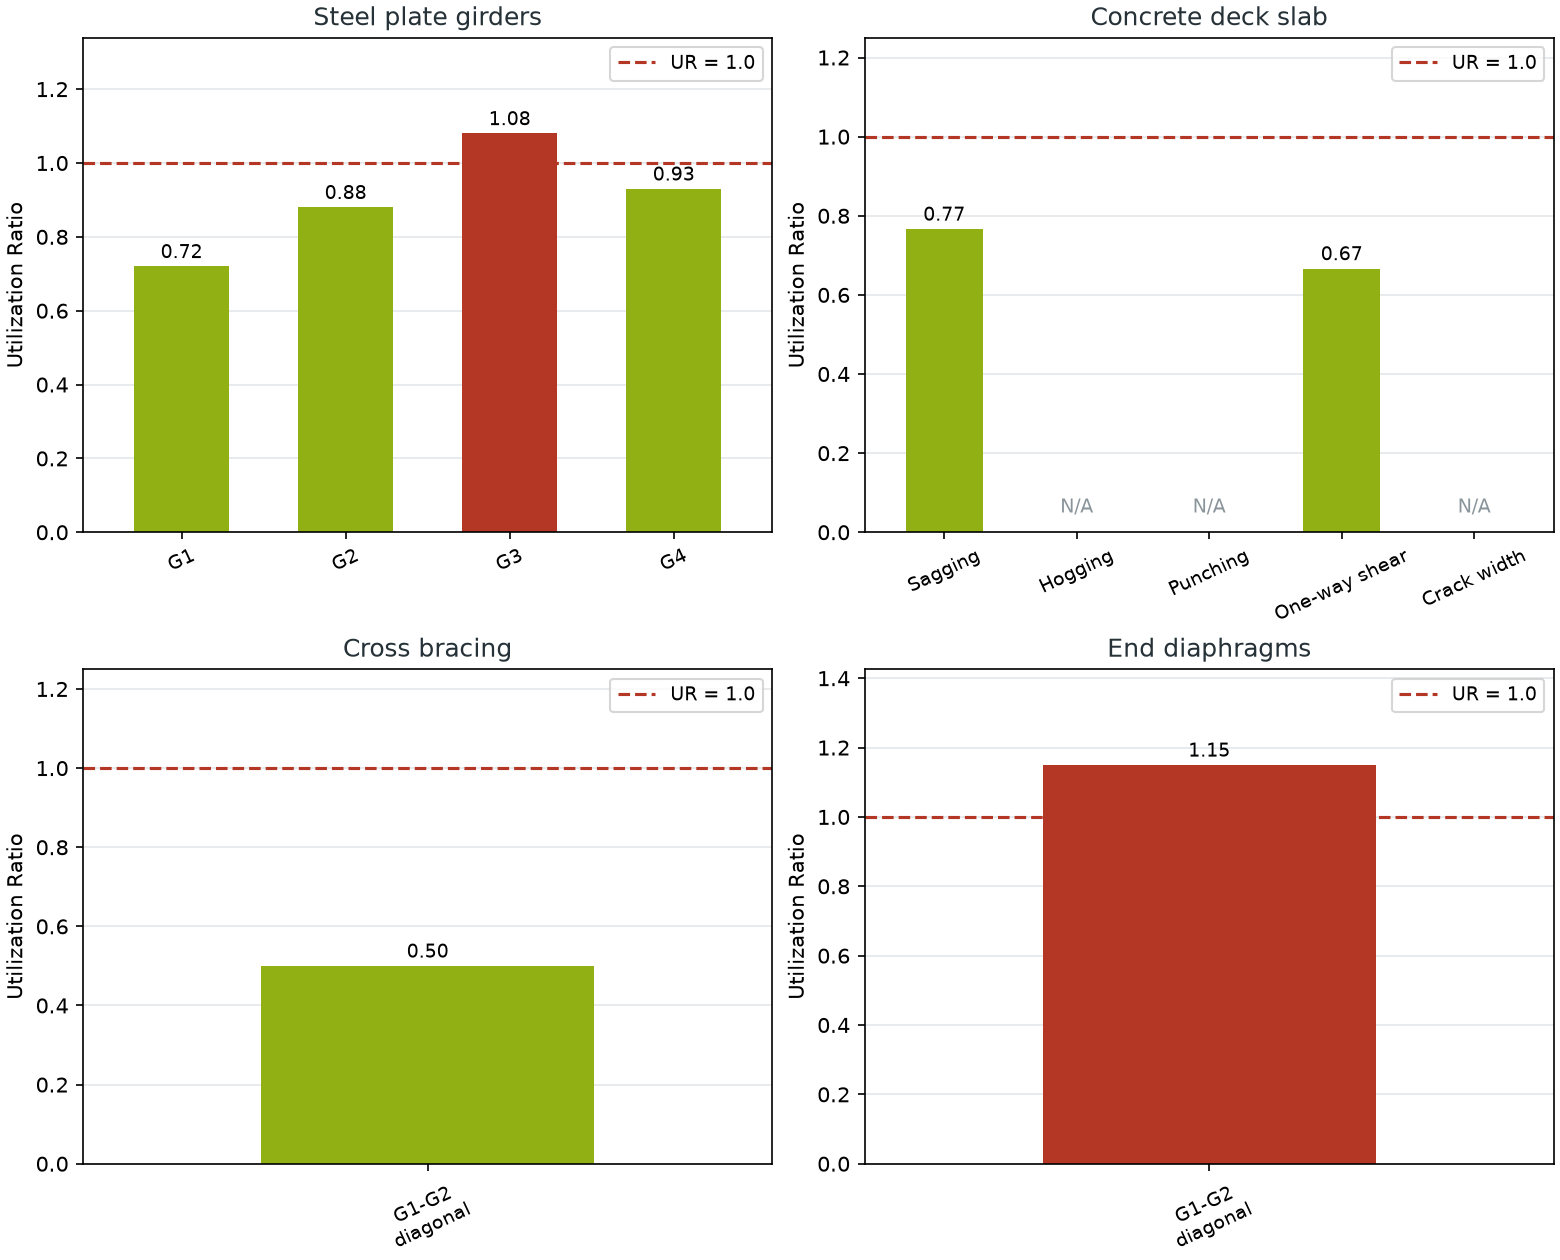
\includegraphics[width=0.98\linewidth]{Report_After_assets/utilization.png}%
\caption{Utilization ratios from existing design results. The dashed line marks UR = 1.0; N/A means no valid result was supplied. Girder and bracing bars show the highest available check ratio for each member. Refer to individual checks for code{-}specific warning bands.}%
\end{figure}

\ReportTableGap
\begingroup
\ReportTableSetup
\ReportTableFont
\begin{longtable}{|C{3.4000cm}|L{4.5000cm}|C{2.3000cm}|C{2.3000cm}|>{\centering\arraybackslash}p{1.6000cm}|}
\caption{\textbf{Overall Design Check Summary --- All Members}}\\
\hline
\textbf{Member / Check} & \textbf{Governing Load Combo} & \textbf{Demand} & \textbf{Capacity} & \textbf{UR} \\[\ReportRowGap]
\hline
\endfirsthead
\hline
\textbf{Member / Check} & \textbf{Governing Load Combo} & \textbf{Demand} & \textbf{Capacity} & \textbf{UR} \\[\ReportRowGap]
\hline
\endhead
\hline
\endfoot
\hline
\endlastfoot

Girder --- Moment & N/A & 108.00 kNm & 100.00 kNm & \textcolor{reportFail}{1.08} \\[\ReportRowGap]
\hline
Girder --- Shear & N/A & N/A & N/A & N/A \\[\ReportRowGap]
\hline
Girder --- LTB (constr.) & N/A & N/A & N/A & N/A \\[\ReportRowGap]
\hline
Girder --- Deflection & N/A & N/A & N/A & N/A \\[\ReportRowGap]
\hline
Girder --- Stress & N/A & N/A & N/A & N/A \\[\ReportRowGap]
\hline
Girder --- Fatigue & N/A & N/A & N/A & N/A \\[\ReportRowGap]
\hline
Transverse Shear (slab) & N/A & N/A & N/A & N/A \\[\ReportRowGap]
\hline
Crack Width (slab) & Frequent SLS & N/A & N/A & N/A \\[\ReportRowGap]
\hline
Deck --- Flexure (sagging) & Basic ULS: 0DL + 0LL & 92.00 kN-m/m & 120.00 kN-m/m & 0.77 \\[\ReportRowGap]
\hline
Deck --- Flexure (hogging) & Basic ULS: 0DL + 0LL & N/A & N/A & N/A \\[\ReportRowGap]
\hline
Deck --- Cantilever Overhang & Basic ULS: 0DL + 0LL & N/A & N/A & N/A \\[\ReportRowGap]
\hline
Deck --- Punching Shear & Basic ULS: 0DL + 0LL & N/A & N/A & N/A \\[\ReportRowGap]
\hline
Deck --- One-Way Shear & Basic ULS: 0DL + 0LL & 120.00 kN/m & 180.00 kN/m & 0.67 \\[\ReportRowGap]
\hline
Cross Bracing --- Compression & Synthetic ULS & 50.00 kN & 100.00 kN & 0.50 \\[\ReportRowGap]
\hline
Cross Bracing --- Tension & N/A & N/A & N/A & N/A \\[\ReportRowGap]
\hline
Cross Bracing --- Slenderness & N/A & 120.0 & 250 & 0.48 \\[\ReportRowGap]
\hline
End Diaphragm --- Compression & Synthetic ULS & 115.00 kN & 100.00 kN & \textcolor{reportFail}{1.15} \\[\ReportRowGap]
\hline
End Diaphragm --- Tension & N/A & N/A & N/A & N/A \\[\ReportRowGap]
\hline
\end{longtable}
\endgroup
\noindent\textit{Note: UR = Demand / Capacity. The unity line is a visual reference; supplied backend statuses retain the code-specific acceptance rules. The governing check for each component is highlighted in the individual design check sections above.}


\setcounter{chapter}{5}
\chapter{Drawings and Visualizations}
\label{ch:drawings}

This section presents CAD-generated views of the designed bridge and its components. All views are generated automatically by OsdagBridge using pythonOCC.

\section{Bridge Configuration and Layout}
\label{sec:bridge-layout}

\noindent\textit{Unavailable: Overall 3D Bridge Superstructure. No drawing was supplied.}\par


\noindent\textit{Unavailable: Typical Cross Section. No drawing was supplied.}\par


\noindent\textit{Unavailable: Top View. No drawing was supplied.}\par


\section{Plate Girder --- Detailed Views}
\label{sec:girder-views}

\noindent\textit{Unavailable: 3D View of Plate Girders. No drawing was supplied.}\par


\noindent\textit{Unavailable: Cross Section of Plate Girder. No drawing was supplied.}\par


\noindent\textit{Unavailable: Side View of Girder. No drawing was supplied.}\par


\section{Cross Bracing Detail}
\label{sec:bracing-detail}

\noindent\textit{Unavailable: Cross Bracing Layout. No drawing was supplied.}\par


\noindent
\begin{minipage}[t]{0.31\textwidth}\textit{Unavailable: Cross Bracing -- Bracing Section.}\end{minipage}
\hfill
\begin{minipage}[t]{0.31\textwidth}\textit{Unavailable: Cross Bracing -- Top Chord Section.}\end{minipage}
\hfill
\begin{minipage}[t]{0.31\textwidth}\textit{Unavailable: Cross Bracing -- Bottom Chord Section.}\end{minipage}
            

\section{End Diaphragm Detail}
\label{sec:diaphragm-detail}

\noindent\textit{Unavailable: End Diaphragm Layout. No drawing was supplied.}\par


\noindent
\begin{minipage}[t]{0.31\textwidth}\textit{Unavailable: End Diaphragm -- Bracing Section.}\end{minipage}
\hfill
\begin{minipage}[t]{0.31\textwidth}\textit{Unavailable: End Diaphragm -- Top Chord Section.}\end{minipage}
\hfill
\begin{minipage}[t]{0.31\textwidth}\textit{Unavailable: End Diaphragm -- Bottom Chord Section.}\end{minipage}


\setcounter{chapter}{6}
\chapter{Material Take-off \& Quantity Summary}
\label{ch:material-takeoff}

\noindent\textbf{Table 7.1  Bill of Materials (Steel, Concrete, and Reinforcement Quantities)}

\begingroup

\begingroup
\ReportTableSetup
\ReportTableFont
\begin{longtable}{|C{1.0000cm}|L{3.8000cm}|C{2.6000cm}|C{1.8000cm}|C{1.8000cm}|C{1.8000cm}|C{1.8000cm}|}
\hline
\textbf{S.N.} & \textbf{Item Description} & \textbf{Volume} & \textbf{Quantity} & \textbf{Total Volume} & \textbf{Weight (MT)} & \textbf{Total Weight (MT)} \\
\hline
\endfirsthead
\hline
\textbf{S.N.} & \textbf{Item Description} & \textbf{Volume} & \textbf{Quantity} & \textbf{Total Volume} & \textbf{Weight (MT)} & \textbf{Total Weight (MT)} \\
\hline
\endhead
\hline
\endfoot
\hline
\endlastfoot

1 & Structural Steel for Girders & $0.06000\text{ m}^2 \times 25.00\text{ m} = 1.50000\text{ m}^3$ & 4 & 6.00 & 11.78 & 47.10 \\
\hline
2(a) & Cross Bracing - Top Chord & N/A & N/A & N/A & N/A & N/A \\
\hline
2(b) & Cross Bracing - Bottom Chord & N/A & N/A & N/A & N/A & N/A \\
\hline
2(c) & Cross Bracing - Diagonal Chord & N/A & N/A & N/A & N/A & N/A \\
\hline
2(d) & End Diaphragms & N.A. & N.A. & N.A. & N.A. & N.A. \\
\hline
3 & Concrete for Deck Slab & $10.50\text{ m} \times 0.25\text{ m} \times 25.00\text{ m} = 65.62\text{ m}^3$ & 1 & 65.62 & 164.06 & 164.06 \\
\hline
4 & Reinforcement Steel & $0.040127\text{ m}^2 \times 25.00\text{ m} = 1.00318\text{ m}^3$ & 1 & 1.00 & 7.88 & 7.88 \\
\hline
5 & Shear Stud Connectors & N/A & N/A & N/A & N/A & N/A \\
\hline
6 & Crash Barrier & N/A & N/A & N/A & N/A & N/A \\
\hline
\end{longtable}
\endgroup
\endgroup
\noindent\textit{Quantities reproduce the existing bill of quantities. End diaphragm mass is N/A unless explicitly supplied; it is not inferred from cross bracing. Reinforcement tonnage in the upstream bill of quantities is an estimate of 120 kg per cubic metre of deck concrete, not a reinforcement schedule.}
\begin{figure}[htbp]%
\centering%
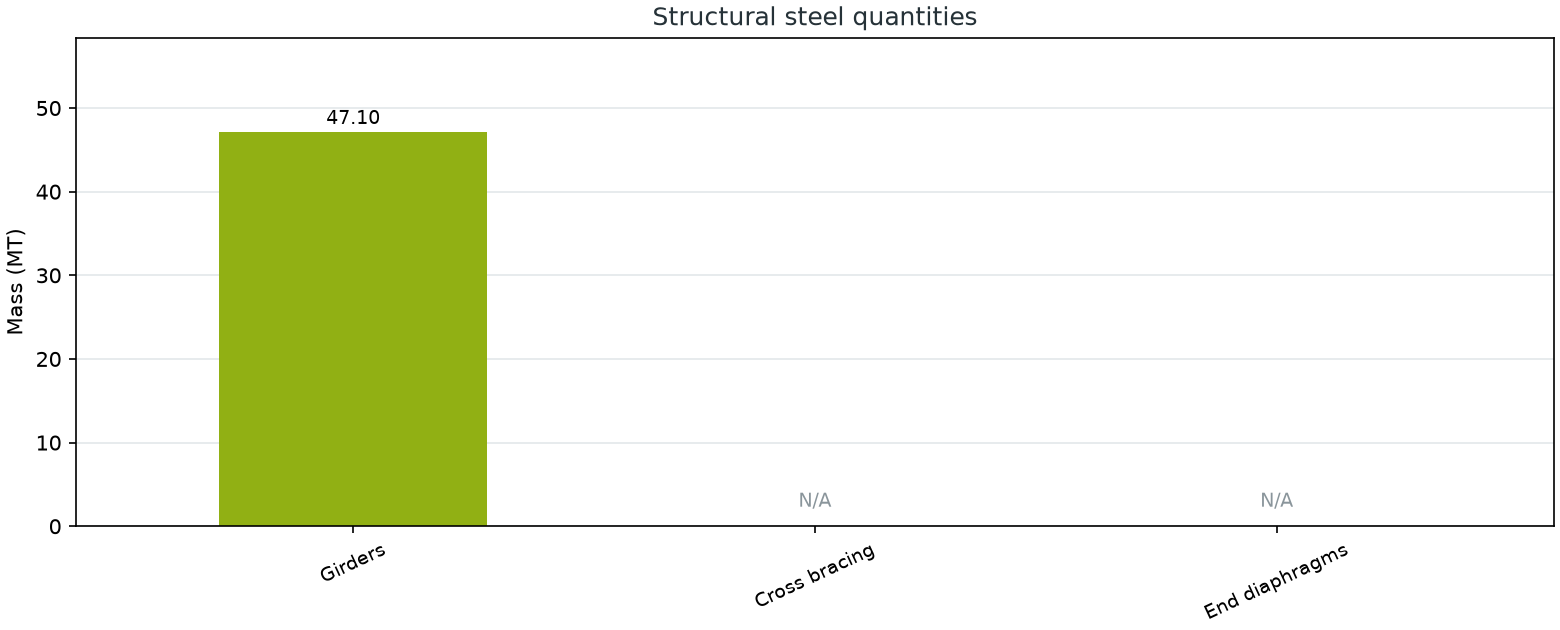
\includegraphics[width=0.98\linewidth]{Report_After_assets/steel_quantities.png}%
\caption{Structural steel quantities in metric tonnes. N/A denotes unavailable quantities.}%
\end{figure}\begin{figure}[htbp]%
\centering%
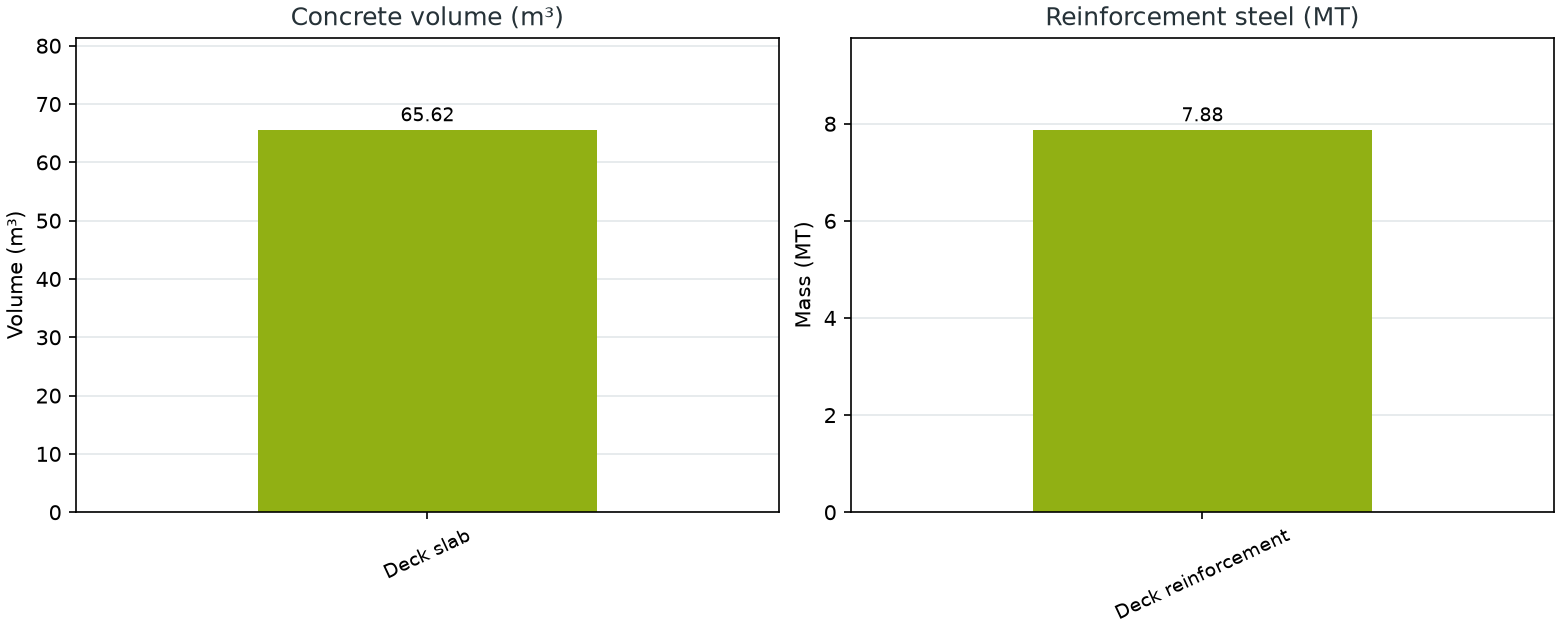
\includegraphics[width=0.98\linewidth]{Report_After_assets/deck_quantities.png}%
\caption{Deck concrete volume and estimated reinforcement mass, displayed on separate axes because their units differ.}%
\end{figure}
\setcounter{chapter}{7}
\chapter{Standards \& Assumptions}
\label{ch:Design Standards}

This section provides references to standards used to calibrate the OsdagBridge
design modules, and notes the limitations of the current software version.

\section{Design Standards}
\label{sec:design_standards}

The following Indian Road Congress (IRC) codes and Indian Standards (IS) 
form the basis of all design calculations in this software.

\ReportTableGap


\begingroup
\ReportTableSetup
\ReportTableFont
\begin{longtable}{|C{1.9131cm}|C{1.9131cm}|p{12.4350cm}|}

\caption{\textbf{IRC Codes}}\\

\hline
\textbf{Code} & \textbf{Year} & \textbf{Title / Scope} \\ 
\hline
\endfirsthead
\hline
\textbf{Code} & \textbf{Year} & \textbf{Title / Scope} \\ 
\hline
\endhead
\hline
\endfoot
\hline
\endlastfoot

IRC 5 & 2015 & General Features of Design - carriageway widths, kerb, footpath dimensions \\ 
\hline
IRC 6 & 2017 & Loads and Load Combinations - dead load, live load, impact, wind, temperature, etc. \\ 
\hline
IRC 22 & 2015 & Composite Construction (LS) - Composite section properties, ULS/SLS design, shear connectors \\ 
\hline
IRC 24 & 2010 & Steel Road Bridges (LS) - Stiffener design, skew angle limits, diaphragm requirements \\ 
\hline
IRC 112 & 2020 & Concrete Road Bridges - Deck slab flexure, shear, crack width, reinforcement \\ 
\hline
IRC SP 114 & 2018 & Seismic Design of Road Bridges \\ 
\hline
\end{longtable}
\endgroup



\begingroup
\ReportTableSetup
\ReportTableFont
\begin{longtable}{|C{1.9131cm}|C{1.9131cm}|p{12.4350cm}|}

\caption{\textbf{IS Codes}}\\

\hline
\textbf{Code} & \textbf{Year} & \textbf{Scope} \\
\hline
\endfirsthead
\hline
\textbf{Code} & \textbf{Year} & \textbf{Scope} \\
\hline
\endhead
\hline
\endfoot
\hline
\endlastfoot

IS 800 & 2007 & Steel construction - tension, compression, bending, shear, LTB, stiffeners, combined checks \\
\hline
IS 456 & 2000 & Concrete - simplified stress-block for deck moment capacity \\
\hline
IS 1786 & 2008 & Reinforcement steel properties \\
\hline
IS 1893 (Part 3) & 2014 & Earthquake resistant design \\
\hline
IS 2062 & 2011 & Structural steel - yield and ultimate strength by grade \\
\hline
\end{longtable}
\endgroup


\clearpage
\section{Analysis and Design Assumptions of This Version}
\label{sec:design-assumptions}

\textbf{Structural Analysis}

\begin{itemize}
    \item All girders are modelled as simply supported; continuous spans are not currently supported.
    \item A 3D grillage model (OSPGrillage) is used for load distribution. Grillage members carry composite section properties after the construction stage.
    \item The transverse member forces are computed using an approximate 2D frame analogy. For irregular or skewed geometries, a 3D FEM is recommended.
    \item Fixed bearing stiffness is modelled as $k = 1{,}000{,}000 \,\text{kN/m}$ (virtually rigid); free/expansion bearing as $k = 100 \, \text{kN/m}$.
    \item Construction stage sequence analysis is approximate. Detailed staged analysis should be performed for long-term deflection checks.
\end{itemize}

\textbf{Composite Action}

\begin{itemize}
    \item Full shear connection is assumed at ULS with headed stud connectors designed per IRC 22:2015 Cl.606.
    \item Short-term composite section properties (modular ratio $n = E_s/E_{cm}$) are used for ULS checks.
    \item Long-term composite section properties (with creep-adjusted modular ratio) are used for SLS deflection and crack-width checks.
    \item Pre-composite stage: the steel girder alone resists all construction loads prior to concrete gaining strength.
\end{itemize}


\textbf{Material Properties (IRC 22:2015 Annex III)}

\begin{itemize}
\item Steel: $E_s = 200{,}000 \, \text{MPa}, \ G_s = 80{,}000 \, \text{MPa}, \ \nu = 0.30, \ \alpha = 11.7 \times 10^{-6}/^\circ\mathrm{C}$ (grade-independent).
\item Minimum structural concrete grade: M25.
\item Default reinforcement grade: Fe500.
\end{itemize}

\textbf{Partial Safety Factors (IRC 22:2015 Cl.601.4)}

\begin{itemize}
\item $\gamma_{m0}$ (steel yield, ULS) = 1.10
\item $\gamma_{m1}$ (steel ultimate, ULS) = 1.25
\item Reinforcement (ULS) = 1.15
\item Welds -- shop: 1.25; field: 1.50
\item Fatigue ($\gamma_{mft}$) = 1.35
\end{itemize}

\textbf{Loading}

\begin{itemize}
\item Dead load densities per IRC 6:2017 Cl.203: structural steel $78.5 \ \text{kN/m}^3$, concrete $25.0 \ \text{kN/m}^3$, bituminous wearing course $24.0 \ \text{kN/m}^3$.
\item Multi-lane live load reduction factors per IRC 6:2017 Cl.204.4 Table 6A: 1st lane = 1.0, 2nd lane = 0.8, 3rd lane onwards = 0.4.
\item Impact factor (dynamic load allowance) computed from span per IRC 6:2017 Cl.208.2/208.3.
\item Wind load applied as transverse, longitudinal, and vertical components per IRC 6:2017, clauses 209.3.3 to 209.3.5.
\end{itemize}

\textbf{Serviceability Limits}

\begin{itemize}
\item Deflection limits (IRC 22:2015 Cl.604.3.2): live load + impact $\leq L/800$; total $\leq L/600$.
\item SLS stress limits: concrete $\sigma_c \leq 0.48 f_{ck}$; rebar $\sigma_s \leq 0.80 f_{yk}$; steel $f_e \leq 0.9 f_y$.
\item Permissible crack width: $w_k \leq 0.3 \ \text{mm}$ (bridge deck, exposure class XS2/XD2 per IRC 112:2020 Cl.12.3.2).
\end{itemize}

\textbf{Fatigue}

\begin{itemize}
\item Reference fatigue life: $N_{sc} = 2 \times 10^6$ cycles (IRC 22:2015 Cl.605).
\item Constant stress range is assumed. A thickness correction factor $\mu_r$ is applied for plate thickness $> 25 \ \text{mm}$.
\end{itemize}

\textbf{Stiffener Design}

\begin{itemize}
\item Intermediate transverse stiffener and bearing stiffener design follows IS 800:2007 Cl.8.7.2/8.7.3 and IRC 24:2010 Cl.509.7.2/509.7.3.
\end{itemize}


\section{Known Limitations of This Version}
\label{sec:limitations}

\begin{itemize}
\item Substructure (piers, pile caps, foundations) and bearing design are not included.
\item Splice connection design is not implemented.
\item Skew angle $>$ 15 degrees requires independent manual analysis (IRC 24 Cl. 504.8).
\item Construction stage sequence analysis is approximate; detailed staged analysis
  should be performed for long-term deflection checks.
\item The grillage analysis assumes simply supported boundary conditions;
  continuous spans are not currently supported.
\end{itemize}


\chapter*{References}
\addcontentsline{toc}{chapter}{References}


\begin{enumerate}

\item IRC 5 (2024) --- \textit{Standard Specifications and Code of Practice for Road Bridges, Section I: General Features of Design.}

\item IRC 6 (2017) --- \textit{Standard Specifications and Code of Practice for Road Bridges, Section II: Loads and Load Combinations.}

\item IRC 22 (2014) --- \textit{Standard Specifications and Code of Practice for Road Bridges, Section VI: Composite Construction (Limit State Design).}

\item IRC 24 (2010) --- \textit{Standard Specifications and Code of Practice for Road Bridges, Section V: Steel Road Bridges (Limit State Method).}

\item IRC 112 (2011) --- \textit{Code of Practice for Concrete Road Bridges.}

\item IRC SP 114 (2018) --- \textit{Guidelines for Seismic Design of Road Bridges.}

\item IS 800 (2007) --- \textit{Indian Standard: General Construction in Steel --- Code of Practice.}

\item IS 2062 (2011) --- \textit{Hot Rolled Medium and High Tensile Structural Steel --- Specification.}

\item Subramanian, N. (2008). \textit{Design of Steel Structures.} Oxford University Press.

\item Steel-INSDAG Teaching Resource Materials. \url{https://www.steel-insdag.org}

\end{enumerate}

\end{document}